At this stage in the workflow, after converting raw reads to
interpretable species abundances, and after filtering and transforming
these abundances to focus attention on scientifically meaningful
quantities, we are in a position to consider more careful statistical
analysis. R is an ideal environment for performing these analyses, as
it has an active community of package developers building simple
interfaces to sophisticated techniques. As a variety of methods are
available, there is no need to commit to any rigid analysis strategy a
priori. Further, the ability to easily call packages without
reimplementing methods frees researchers to iterate rapidly through
alternative analysis ideas. The advantage of performing this full
workflow in R is that this transition from bioinformatics to
statistics is effortless.

We back these claims by illustrating several analysis on the mouse
data prepared above. We experiment with several flavors of exploratory
ordination before shifting to more formal testing and modeling,
explaining the settings in which the different points of view are most
appropriate. Finally, we provide example analysis of multitable data,
using a study in which both metabolomic and microbial abundance
measurements were collected on the same samples, to demonstrate that
the general workflow presented here can be adapted to the multitable
setting.



\begin{knitrout}
\definecolor{shadecolor}{rgb}{0.969, 0.969, 0.969}\color{fgcolor}\begin{kframe}
\begin{alltt}
\hlstd{.cran_packages}  \hlkwb{<-}  \hlkwd{c}\hlstd{(}\hlstr{"knitr"}\hlstd{,} \hlstr{"phyloseqGraphTest"}\hlstd{,} \hlstr{"phyloseq"}\hlstd{,} \hlstr{"shiny"}\hlstd{,}
                    \hlstr{"miniUI"}\hlstd{,} \hlstr{"caret"}\hlstd{,} \hlstr{"pls"}\hlstd{,} \hlstr{"e1071"}\hlstd{,} \hlstr{"ggplot2"}\hlstd{,} \hlstr{"randomForest"}\hlstd{,}
                    \hlstr{"vegan"}\hlstd{,} \hlstr{"plyr"}\hlstd{,} \hlstr{"dplyr"}\hlstd{,} \hlstr{"ggrepel"}\hlstd{,} \hlstr{"nlme"}\hlstd{,}
                    \hlstr{"reshape2"}\hlstd{,} \hlstr{"devtools"}\hlstd{,} \hlstr{"PMA"}\hlstd{,}\hlstr{"structSSI"}\hlstd{,}\hlstr{"ade4"}\hlstd{,}
                    \hlstr{"igraph"}\hlstd{,} \hlstr{"ggnetwork"}\hlstd{,} \hlstr{"intergraph"}\hlstd{,} \hlstr{"scales"}\hlstd{)}
\hlstd{.github_packages} \hlkwb{<-} \hlkwd{c}\hlstd{(}\hlstr{"jfukuyama/phyloseqGraphTest"}\hlstd{)}
\hlstd{.bioc_packages} \hlkwb{<-} \hlkwd{c}\hlstd{(}\hlstr{"phyloseq"}\hlstd{,} \hlstr{"genefilter"}\hlstd{,} \hlstr{"impute"}\hlstd{)}

\hlcom{# Install CRAN packages (if not already installed)}
\hlstd{.inst} \hlkwb{<-} \hlstd{.cran_packages} \hlopt \hlkwd{installed.packages}\hlstd{()}
\hlkwa{if} \hlstd{(}\hlkwd{any}\hlstd{(}\hlopt{!}\hlstd{.inst)) \{}
  \hlkwd{install.packages}\hlstd{(.cran_packages[}\hlopt{!}\hlstd{.inst],} \hlkwc{repos} \hlstd{=} \hlstr{"http://cran.rstudio.com/"}\hlstd{)}
\hlstd{\}}

\hlstd{.inst} \hlkwb{<-} \hlstd{.github_packages} \hlopt \hlkwd{installed.packages}\hlstd{()}
\hlkwa{if} \hlstd{(}\hlkwd{any}\hlstd{(}\hlopt{!}\hlstd{.inst)) \{}
  \hlstd{devtools}\hlopt{::}\hlkwd{install_github}\hlstd{(.github_packages[}\hlopt{!}\hlstd{.inst])}
\hlstd{\}}

\hlstd{.inst} \hlkwb{<-} \hlstd{.bioc_packages} \hlopt \hlkwd{installed.packages}\hlstd{()}
\hlkwa{if} \hlstd{(}\hlkwd{any}\hlstd{(}\hlopt{!}\hlstd{.inst)) \{}
  \hlkwd{source}\hlstd{(}\hlstr{"http://bioconductor.org/biocLite.R"}\hlstd{)}
  \hlkwd{biocLite}\hlstd{(.bioc_packages[}\hlopt{!}\hlstd{.inst])}
\hlstd{\}}
\end{alltt}
\end{kframe}
\end{knitrout}


\subsubsection*{Preprocessing}

Before doing the multivariate projections, we will add a few columns
to our sample data, which can then be used to annotate plots. From
Figure \ref{fig:preprocessing-setup}, we see that the ages of the mice
come in a couple of groups, and so we make a categorical variable
corresponding to young, middle-aged, and old mice. We also record the
total number of counts seen in each sample and log-transform the data
as an approximate variance stabilizing transformation.


\begin{figure}[H]
\begin{knitrout}
\definecolor{shadecolor}{rgb}{0.969, 0.969, 0.969}\color{fgcolor}\begin{kframe}
\begin{alltt}
\hlkwd{qplot}\hlstd{(}\hlkwd{sample_data}\hlstd{(ps)}\hlopt{$}\hlstd{age,} \hlkwc{geom} \hlstd{=} \hlstr{"histogram"}\hlstd{)} \hlopt{+} \hlkwd{xlab}\hlstd{(}\hlstr{"age"}\hlstd{)}
\hlkwd{qplot}\hlstd{(}\hlkwd{log10}\hlstd{(}\hlkwd{rowSums}\hlstd{(}\hlkwd{otu_table}\hlstd{(ps))))} \hlopt{+}
  \hlkwd{xlab}\hlstd{(}\hlstr{"Logged counts-per-sample"}\hlstd{)}
\end{alltt}
\end{kframe}

{\centering \includegraphics[width=\maxwidth]{analysisfigure/preprocessing-plot-1} 
\includegraphics[width=\maxwidth]{analysisfigure/preprocessing-plot-2} 

}



\end{knitrout}
\caption{Preliminary plots suggest certain preprocessing steps. The
  histogram on the left motivates the creation of a new categorical
  variable, binning age into one of the three peaks. The histogram on
  the right suggests that a $\log\left(1 + x\right)$ transformation is
  sufficient for normalizing the abundance data.}
\label{fig:preprocessing-setup}
\end{figure}

For a first pass, we look at principal coordinates analysis (PCoA) with
either the Bray-Curtis dissimilarity on the weighted Unifrac
distance. We see immediately that there are six outliers. These turn
out to be the samples from females 5 and 6 on day 165 and the samples
from males 3, 4, 5, and 6 on day 175. We will take them out, since we
are mainly interested in the relationships between the non-outlier
points.
\begin{knitrout}
\definecolor{shadecolor}{rgb}{0.969, 0.969, 0.969}\color{fgcolor}\begin{kframe}
\begin{alltt}
\hlstd{pslog} \hlkwb{<-} \hlkwd{transform_sample_counts}\hlstd{(ps,} \hlkwa{function}\hlstd{(}\hlkwc{x}\hlstd{)} \hlkwd{log}\hlstd{(}\hlnum{1} \hlopt{+} \hlstd{x))}
\hlkwd{sample_data}\hlstd{(pslog)}\hlopt{$}\hlstd{age_binned} \hlkwb{<-} \hlkwd{cut}\hlstd{(}\hlkwd{sample_data}\hlstd{(pslog)}\hlopt{$}\hlstd{age,}
                                     \hlkwc{breaks} \hlstd{=} \hlkwd{c}\hlstd{(}\hlnum{0}\hlstd{,} \hlnum{100}\hlstd{,} \hlnum{200}\hlstd{,} \hlnum{400}\hlstd{))}
\hlstd{out.wuf.log} \hlkwb{<-} \hlkwd{ordinate}\hlstd{(pslog,} \hlkwc{method} \hlstd{=} \hlstr{"MDS"}\hlstd{,} \hlkwc{distance} \hlstd{=} \hlstr{"wunifrac"}\hlstd{)}
\end{alltt}
\end{kframe}
\end{knitrout}

\begin{figure}[H]
\begin{knitrout}
\definecolor{shadecolor}{rgb}{0.969, 0.969, 0.969}\color{fgcolor}\begin{kframe}
\begin{alltt}
\hlstd{evals} \hlkwb{<-} \hlstd{out.wuf.log}\hlopt{$}\hlstd{values}\hlopt{$}\hlstd{Eigenvalues}
\hlkwd{plot_ordination}\hlstd{(pslog, out.wuf.log,} \hlkwc{color} \hlstd{=} \hlstr{"age_binned"}\hlstd{)} \hlopt{+}
  \hlkwd{labs}\hlstd{(}\hlkwc{col} \hlstd{=} \hlstr{"Binned Age"}\hlstd{)} \hlopt{+}
  \hlkwd{coord_fixed}\hlstd{(}\hlkwd{sqrt}\hlstd{(evals[}\hlnum{2}\hlstd{]} \hlopt{/} \hlstd{evals[}\hlnum{1}\hlstd{]))}
\end{alltt}
\end{kframe}

{\centering \includegraphics[width=\maxwidth]{analysisfigure/outlier-detect-plot-1} 

}



\end{knitrout}
\label{fig:outlier-detect}
\caption{An ordination on the logged abundance data reveals a few
  outliers.}
\end{figure}
Before we continue, we should check the two female
outliers -- they have been taken over by the same OTU/RSV, which has a
relative abundance of over 90\% in each of them. This is the only time
in the entire data set that this RSV has such a high relative
abundance -- the rest of the time it is below 20\%. In particular, its
diversity is by far the lowest of all the samples.


\begin{knitrout}
\definecolor{shadecolor}{rgb}{0.969, 0.969, 0.969}\color{fgcolor}\begin{kframe}
\begin{alltt}
\hlstd{rel_abund} \hlkwb{<-} \hlkwd{t}\hlstd{(}\hlkwd{apply}\hlstd{(}\hlkwd{otu_table}\hlstd{(ps),} \hlnum{1}\hlstd{,} \hlkwa{function}\hlstd{(}\hlkwc{x}\hlstd{) x} \hlopt{/} \hlkwd{sum}\hlstd{(x)))}
\hlkwd{qplot}\hlstd{(rel_abund[,} \hlnum{12}\hlstd{],} \hlkwc{geom} \hlstd{=} \hlstr{"histogram"}\hlstd{)} \hlopt{+}
  \hlkwd{xlab}\hlstd{(}\hlstr{"Relative abundance"}\hlstd{)}
\end{alltt}
\end{kframe}
\end{knitrout}
\begin{figure}[H]
\includegraphics[height=0.2\linewidth]{analysisfigure/outlier-analyze-1}
\caption{The outlier samples are dominated by a single RSV.}
\label{fig:outlier-analysize}
\end{figure}

\subsubsection*{Aspect ratio of ordination plots}
In the above plots, you may have noticed as did the reviewers of the first version of the paper, that
the maps are not presented as square representations as is often the case in
standard PCoA and PCA plots in the literature.

The reason for this is that as we are trying to represent the distances between samplesas faitfully as possible
we have to take into account that the second eigenvalue is always smaller
than the first, sometimes considerably so, thus we normalize the axis ration to the relevant eigenvalue
ratios.

\subsection*{Different Ordination Projections}

As we have seen, an important first step in analyzing microbiome data is to do
unsupervised, exploratory analysis. This is simple to do in
\BioCpkg{phyloseq}, which provides many distances and ordination
methods.

After documenting the outliers, we are going to compute ordinations
with these outliers removed and more carefully study the output. We
see that there is a fairly substantial age effect that is consistent
between all the mice, male and female, and from different
litters. We'll first perform a PCoA using Bray-Curtis dissimilarity.

The first plot shows the ordination of the samples, and we see that
the second axis corresponds to an age effect, with the samples from
the younger and older mice separating fairly well. The first axis
correlates fairly well with library size (this is not shown).
The first axis explains about twice the variability than the first,
this translates into the elongated form of the ordination plot.

\begin{knitrout}
\definecolor{shadecolor}{rgb}{0.969, 0.969, 0.969}\color{fgcolor}\begin{kframe}
\begin{alltt}
\hlkwd{setup_example}\hlstd{(}\hlkwd{c}\hlstd{(}\hlstr{"phyloseq"}\hlstd{,} \hlstr{"ggplot2"}\hlstd{,} \hlstr{"plyr"}\hlstd{,} \hlstr{"dplyr"}\hlstd{,} \hlstr{"reshape2"}\hlstd{,}
                \hlstr{"ade4"}\hlstd{,} \hlstr{"ggrepel"}\hlstd{))}
\hlstd{out.bc.log} \hlkwb{<-} \hlkwd{ordinate}\hlstd{(pslog,} \hlkwc{method} \hlstd{=} \hlstr{"MDS"}\hlstd{,} \hlkwc{distance} \hlstd{=} \hlstr{"bray"}\hlstd{)}
\end{alltt}
\end{kframe}
\end{knitrout}

\begin{figure}[H]
\begin{knitrout}
\definecolor{shadecolor}{rgb}{0.969, 0.969, 0.969}\color{fgcolor}\begin{kframe}
\begin{alltt}
\hlstd{evals} \hlkwb{<-} \hlstd{out.bc.log}\hlopt{$}\hlstd{values}\hlopt{$}\hlstd{Eigenvalues}
\hlkwd{plot_ordination}\hlstd{(pslog, out.bc.log,} \hlkwc{color} \hlstd{=} \hlstr{"age_binned"}\hlstd{)} \hlopt{+}
  \hlkwd{coord_fixed}\hlstd{(}\hlkwd{sqrt}\hlstd{(evals[}\hlnum{2}\hlstd{]} \hlopt{/} \hlstd{evals[}\hlnum{1}\hlstd{]))} \hlopt{+}
  \hlkwd{labs}\hlstd{(}\hlkwc{col} \hlstd{=} \hlstr{"Binned Age"}\hlstd{)}
\end{alltt}
\end{kframe}

{\centering \includegraphics[width=\maxwidth]{analysisfigure/ordinations-bray-plot-1} 

}



\end{knitrout}
\caption{A PCoA plot using Bray-Curtis distance between samples.}
\label{fig:ordinations-bray}
\end{figure}

Next we look at double principal coordinates analysis (DPCoA)
\cite{Pavoine:2004,Purdom2010,Fukuyama:2012}, which is a phylogenetic ordination method and
that provides a biplot representation of both samples and taxonomic categories. We see
again that the second axis corresponds to young vs. old
mice, and the biplot suggests an interpretation of the second
axis: samples that have larger scores on the second axis have more
taxa from Bacteroidetes and one subset of Firmicutes.

\begin{knitrout}
\definecolor{shadecolor}{rgb}{0.969, 0.969, 0.969}\color{fgcolor}\begin{kframe}
\begin{alltt}
\hlstd{out.dpcoa.log} \hlkwb{<-} \hlkwd{ordinate}\hlstd{(pslog,} \hlkwc{method} \hlstd{=} \hlstr{"DPCoA"}\hlstd{)}
\end{alltt}
\end{kframe}
\end{knitrout}

\begin{figure}
\begin{knitrout}
\definecolor{shadecolor}{rgb}{0.969, 0.969, 0.969}\color{fgcolor}\begin{kframe}
\begin{alltt}
\hlstd{evals} \hlkwb{<-} \hlstd{out.dpcoa.log}\hlopt{$}\hlstd{eig}
\hlkwd{plot_ordination}\hlstd{(pslog, out.dpcoa.log,} \hlkwc{color} \hlstd{=} \hlstr{"age_binned"}\hlstd{,}
                \hlkwc{shape} \hlstd{=} \hlstr{"family_relationship"}\hlstd{)} \hlopt{+}
  \hlkwd{coord_fixed}\hlstd{(}\hlkwd{sqrt}\hlstd{(evals[}\hlnum{2}\hlstd{]} \hlopt{/} \hlstd{evals[}\hlnum{1}\hlstd{]))} \hlopt{+}
  \hlkwd{labs}\hlstd{(}\hlkwc{col} \hlstd{=} \hlstr{"Binned Age"}\hlstd{,} \hlkwc{shape} \hlstd{=} \hlstr{"Litter"}\hlstd{)}
\end{alltt}
\end{kframe}

{\centering \includegraphics[width=\maxwidth]{analysisfigure/ordinations-dpcoa-plot-1} 

}



\end{knitrout}
\caption{A DPCoA plot incorporates phylogenetic information, but is
  dominated by the first axis.}
\label{fig:ordinations-dpcoa}
\end{figure}

\begin{figure}
\begin{knitrout}
\definecolor{shadecolor}{rgb}{0.969, 0.969, 0.969}\color{fgcolor}\begin{kframe}
\begin{alltt}
\hlkwd{plot_ordination}\hlstd{(pslog, out.dpcoa.log,} \hlkwc{type} \hlstd{=} \hlstr{"species"}\hlstd{,} \hlkwc{color} \hlstd{=} \hlstr{"Phylum"}\hlstd{)} \hlopt{+}
  \hlkwd{coord_fixed}\hlstd{(}\hlkwd{sqrt}\hlstd{(evals[}\hlnum{2}\hlstd{]} \hlopt{/} \hlstd{evals[}\hlnum{1}\hlstd{]))}
\end{alltt}
\end{kframe}

{\centering \includegraphics[width=\maxwidth]{analysisfigure/ordinations-dpcoa-species-1} 

}



\end{knitrout}
\caption{The DPCoA sample positions can be interpreted with respect to
  the species coordinates in this display.}
\label{fig:ordinations-dpcoa-species}
\end{figure}

Finally, we can look at the results of PCoA with weighted Unifrac. As
before, we find that the second axis is associated with an age effect,
which is fairly similar to DPCoA. This is not surprising, because both
are phylogenetic ordination methods taking abundance into
account. However, when we compare biplots, we see that the DPCoA
gave a much cleaner interpretation of the second axis, compared to
weighted Unifrac.

\begin{knitrout}
\definecolor{shadecolor}{rgb}{0.969, 0.969, 0.969}\color{fgcolor}\begin{kframe}
\begin{alltt}
\hlstd{out.wuf.log} \hlkwb{<-} \hlkwd{ordinate}\hlstd{(pslog,} \hlkwc{method} \hlstd{=} \hlstr{"PCoA"}\hlstd{,} \hlkwc{distance} \hlstd{=}\hlstr{"wunifrac"}\hlstd{)}
\end{alltt}
\end{kframe}
\end{knitrout}

\begin{figure}
\begin{knitrout}
\definecolor{shadecolor}{rgb}{0.969, 0.969, 0.969}\color{fgcolor}\begin{kframe}
\begin{alltt}
\hlstd{evals} \hlkwb{<-} \hlstd{out.wuf.log}\hlopt{$}\hlstd{values}\hlopt{$}\hlstd{Eigenvalues}
\hlkwd{plot_ordination}\hlstd{(pslog, out.wuf.log,} \hlkwc{color} \hlstd{=} \hlstr{"age_binned"}\hlstd{,}
                \hlkwc{shape} \hlstd{=} \hlstr{"family_relationship"}\hlstd{)} \hlopt{+}
  \hlkwd{coord_fixed}\hlstd{(}\hlkwd{sqrt}\hlstd{(evals[}\hlnum{2}\hlstd{]} \hlopt{/} \hlstd{evals[}\hlnum{1}\hlstd{]))} \hlopt{+}
  \hlkwd{labs}\hlstd{(}\hlkwc{col} \hlstd{=} \hlstr{"Binned Age"}\hlstd{,} \hlkwc{shape} \hlstd{=} \hlstr{"Litter"}\hlstd{)}
\end{alltt}
\end{kframe}

{\centering \includegraphics[width=\maxwidth]{analysisfigure/ordinations-wuf-plot-1} 

}



\end{knitrout}
\caption{The sample positions produced by a PCoA using weighted
  Unifrac.}
\label{fig:ordinations-wuf}
\end{figure}

\begin{figure}
\begin{knitrout}
\definecolor{shadecolor}{rgb}{0.969, 0.969, 0.969}\color{fgcolor}\begin{kframe}
\begin{alltt}
\hlkwd{plot_ordination}\hlstd{(pslog, out.wuf.log,} \hlkwc{type} \hlstd{=} \hlstr{"species"}\hlstd{,} \hlkwc{color} \hlstd{=} \hlstr{"Phylum"}\hlstd{)} \hlopt{+}
  \hlkwd{coord_fixed}\hlstd{(}\hlkwd{sqrt}\hlstd{(evals[}\hlnum{2}\hlstd{]} \hlopt{/} \hlstd{evals[}\hlnum{1}\hlstd{]))}
\end{alltt}
\end{kframe}

{\centering \includegraphics[width=\maxwidth]{analysisfigure/ordinations-wuf-species-1} 

}



\end{knitrout}
\caption{Species coordinates that can be used to interpret the sample
  positions from PCoA with weighted Unifrac. Compared to the
  representation in Figure \ref{fig:ordinations-dpcoa-species}, this
  display is harder to interpret.}
\label{fig:ordinations-wuf-species}
\end{figure}

\subsubsection*{PCA on ranks}

Microbial abundance data is often heavy-tailed, and sometimes it can
be hard to identify a transformation that brings the data to
normality. In these cases, it can be safer to ignore the raw
abundances altogether, and work instead with ranks. We demonstrate
this idea using a rank-transformed version of the data to perform
PCA. First, we create a new matrix, representing the abundances by
their ranks, where the microbe with the smallest in a sample gets
mapped to rank 1, second smallest rank 2, etc.

\begin{knitrout}
\definecolor{shadecolor}{rgb}{0.969, 0.969, 0.969}\color{fgcolor}\begin{kframe}
\begin{alltt}
\hlstd{abund} \hlkwb{<-} \hlkwd{otu_table}\hlstd{(pslog)}
\hlstd{abund_ranks} \hlkwb{<-} \hlkwd{t}\hlstd{(}\hlkwd{apply}\hlstd{(abund,} \hlnum{1}\hlstd{, rank))}
\end{alltt}
\end{kframe}
\end{knitrout}

Naively using these ranks could make differences between pairs of low
and high abundance microbes comparable. In the case where many bacteria are absent or present at trace amounts, an artificially large difference in rank could occur\cite{holmes2011} for minimally abundant taxa.
To avoid this, all those
microbes with rank below some threshold are set to be tied at 1. The ranks for
the other microbes are shifted down, so there is no large gap between
ranks. This transformation is illustrated in Figure
\ref{fig:pca-rank-visualize-procedure}.

\begin{knitrout}
\definecolor{shadecolor}{rgb}{0.969, 0.969, 0.969}\color{fgcolor}\begin{kframe}
\begin{alltt}
\hlstd{abund_ranks} \hlkwb{<-} \hlstd{abund_ranks} \hlopt{-} \hlnum{329}
\hlstd{abund_ranks[abund_ranks} \hlopt{<} \hlnum{1}\hlstd{]} \hlkwb{<-} \hlnum{1}
\end{alltt}
\end{kframe}
\end{knitrout}

\begin{figure}
\begin{knitrout}
\definecolor{shadecolor}{rgb}{0.969, 0.969, 0.969}\color{fgcolor}\begin{kframe}
\begin{alltt}
\hlstd{abund_df} \hlkwb{<-} \hlkwd{melt}\hlstd{(abund,} \hlkwc{value.name} \hlstd{=} \hlstr{"abund"}\hlstd{)} \hlopt
  \hlkwd{left_join}\hlstd{(}\hlkwd{melt}\hlstd{(abund_ranks,} \hlkwc{value.name} \hlstd{=} \hlstr{"rank"}\hlstd{))}
\hlkwd{colnames}\hlstd{(abund_df)} \hlkwb{<-} \hlkwd{c}\hlstd{(}\hlstr{"sample"}\hlstd{,} \hlstr{"seq"}\hlstd{,} \hlstr{"abund"}\hlstd{,} \hlstr{"rank"}\hlstd{)}

\hlstd{abund_df} \hlkwb{<-} \hlkwd{melt}\hlstd{(abund,} \hlkwc{value.name} \hlstd{=} \hlstr{"abund"}\hlstd{)} \hlopt
  \hlkwd{left_join}\hlstd{(}\hlkwd{melt}\hlstd{(abund_ranks,} \hlkwc{value.name} \hlstd{=} \hlstr{"rank"}\hlstd{))}
\hlkwd{colnames}\hlstd{(abund_df)} \hlkwb{<-} \hlkwd{c}\hlstd{(}\hlstr{"sample"}\hlstd{,} \hlstr{"seq"}\hlstd{,} \hlstr{"abund"}\hlstd{,} \hlstr{"rank"}\hlstd{)}

\hlstd{sample_ix} \hlkwb{<-} \hlkwd{sample}\hlstd{(}\hlnum{1}\hlopt{:}\hlkwd{nrow}\hlstd{(abund_df),} \hlnum{8}\hlstd{)}
\hlkwd{ggplot}\hlstd{(abund_df} \hlopt
         \hlkwd{filter}\hlstd{(sample} \hlopt \hlstd{abund_df}\hlopt{$}\hlstd{sample[sample_ix]))} \hlopt{+}
  \hlkwd{geom_point}\hlstd{(}\hlkwd{aes}\hlstd{(}\hlkwc{x} \hlstd{= abund,} \hlkwc{y} \hlstd{= rank,} \hlkwc{col} \hlstd{= sample),}
             \hlkwc{position} \hlstd{=} \hlkwd{position_jitter}\hlstd{(}\hlkwc{width} \hlstd{=} \hlnum{0.2}\hlstd{),} \hlkwc{size} \hlstd{=} \hlnum{.7}\hlstd{)} \hlopt{+}
  \hlkwd{labs}\hlstd{(}\hlkwc{x} \hlstd{=} \hlstr{"Abundance"}\hlstd{,} \hlkwc{y} \hlstd{=} \hlstr{"Thresholded rank"}\hlstd{)} \hlopt{+}
  \hlkwd{scale_color_brewer}\hlstd{(}\hlkwc{palette} \hlstd{=} \hlstr{"Set2"}\hlstd{)}
\end{alltt}
\end{kframe}

{\centering \includegraphics[width=\maxwidth]{analysisfigure/pca-rank-visualize-procedure-1} 

}



\end{knitrout}
\caption{The association between abundance and rank, for a few
  randomly selected samples. The numbers of the $y$-axis are those
  supplied to PCA.}
\label{fig:pca-rank-visualize-procedure}
\end{figure}

We can now perform PCA and study the resulting biplot, given
in Figure \ref{fig:pca-rank-pca-plot}. To produce annotation for this
figure, we used the following block.

\begin{knitrout}
\definecolor{shadecolor}{rgb}{0.969, 0.969, 0.969}\color{fgcolor}\begin{kframe}
\begin{alltt}
\hlstd{ranks_pca} \hlkwb{<-} \hlkwd{dudi.pca}\hlstd{(abund_ranks,} \hlkwc{scannf} \hlstd{= F,} \hlkwc{nf} \hlstd{=} \hlnum{3}\hlstd{)}
\hlstd{row_scores} \hlkwb{<-} \hlkwd{data.frame}\hlstd{(}\hlkwc{li} \hlstd{= ranks_pca}\hlopt{$}\hlstd{li,}
                         \hlkwc{SampleID} \hlstd{=} \hlkwd{rownames}\hlstd{(abund_ranks))}
\hlstd{col_scores} \hlkwb{<-} \hlkwd{data.frame}\hlstd{(}\hlkwc{co} \hlstd{= ranks_pca}\hlopt{$}\hlstd{co,}
                         \hlkwc{seq} \hlstd{=} \hlkwd{colnames}\hlstd{(abund_ranks))}

\hlstd{tax} \hlkwb{<-} \hlkwd{tax_table}\hlstd{(ps)}\hlopt{@}\hlkwc{.Data} \hlopt
  \hlkwd{data.frame}\hlstd{(}\hlkwc{stringsAsFactors} \hlstd{=} \hlnum{FALSE}\hlstd{)}
\hlstd{tax}\hlopt{$}\hlstd{seq} \hlkwb{<-} \hlkwd{rownames}\hlstd{(tax)}

\hlstd{main_orders} \hlkwb{<-} \hlkwd{c}\hlstd{(}\hlstr{"Clostridiales"}\hlstd{,} \hlstr{"Bacteroidales"}\hlstd{,} \hlstr{"Lactobacillales"}\hlstd{,}
                 \hlstr{"Coriobacteriales"}\hlstd{)}
\hlstd{tax}\hlopt{$}\hlstd{Order[}\hlopt{!}\hlstd{(tax}\hlopt{$}\hlstd{Order} \hlopt \hlstd{main_orders)]} \hlkwb{<-} \hlstr{"Other"}
\hlstd{tax}\hlopt{$}\hlstd{Order} \hlkwb{<-} \hlkwd{factor}\hlstd{(tax}\hlopt{$}\hlstd{Order,} \hlkwc{levels} \hlstd{=} \hlkwd{c}\hlstd{(main_orders,} \hlstr{"Other"}\hlstd{))}
\hlstd{tax}\hlopt{$}\hlstd{otu_id} \hlkwb{<-} \hlkwd{seq_len}\hlstd{(}\hlkwd{ncol}\hlstd{(}\hlkwd{otu_table}\hlstd{(ps)))}

\hlstd{row_scores} \hlkwb{<-} \hlstd{row_scores} \hlopt
  \hlkwd{left_join}\hlstd{(}\hlkwd{sample_data}\hlstd{(pslog))}
\hlstd{col_scores} \hlkwb{<-} \hlstd{col_scores} \hlopt
  \hlkwd{left_join}\hlstd{(tax)}
\end{alltt}
\end{kframe}
\end{knitrout}

The results are similar to the
PCoA analyses computed without applying a truncated-ranking
transformation, reinforcing our confidence in the analysis on the
original data.\\
\begin{figure}[h]
\begin{knitrout}
\definecolor{shadecolor}{rgb}{0.969, 0.969, 0.969}\color{fgcolor}\begin{kframe}
\begin{alltt}
\hlstd{evals_prop} \hlkwb{<-} \hlnum{100} \hlopt{*} \hlstd{(ranks_pca}\hlopt{$}\hlstd{eig} \hlopt{/} \hlkwd{sum}\hlstd{(ranks_pca}\hlopt{$}\hlstd{eig))}
\hlkwd{ggplot}\hlstd{()} \hlopt{+}
  \hlkwd{geom_point}\hlstd{(}\hlkwc{data} \hlstd{= row_scores,} \hlkwd{aes}\hlstd{(}\hlkwc{x} \hlstd{= li.Axis1,} \hlkwc{y} \hlstd{= li.Axis2),} \hlkwc{shape} \hlstd{=} \hlnum{2}\hlstd{)} \hlopt{+}
  \hlkwd{geom_point}\hlstd{(}\hlkwc{data} \hlstd{= col_scores,} \hlkwd{aes}\hlstd{(}\hlkwc{x} \hlstd{=} \hlnum{25} \hlopt{*} \hlstd{co.Comp1,} \hlkwc{y} \hlstd{=} \hlnum{25} \hlopt{*} \hlstd{co.Comp2,} \hlkwc{col} \hlstd{= Order),}
             \hlkwc{size} \hlstd{=} \hlnum{.3}\hlstd{,} \hlkwc{alpha} \hlstd{=} \hlnum{0.6}\hlstd{)} \hlopt{+}
  \hlkwd{scale_color_brewer}\hlstd{(}\hlkwc{palette} \hlstd{=} \hlstr{"Set2"}\hlstd{)} \hlopt{+}
  \hlkwd{facet_grid}\hlstd{(}\hlopt{~} \hlstd{age_binned)} \hlopt{+}
  \hlkwd{guides}\hlstd{(}\hlkwc{col} \hlstd{=} \hlkwd{guide_legend}\hlstd{(}\hlkwc{override.aes} \hlstd{=} \hlkwd{list}\hlstd{(}\hlkwc{size} \hlstd{=} \hlnum{3}\hlstd{)))} \hlopt{+}
  \hlkwd{labs}\hlstd{(}\hlkwc{x} \hlstd{=} \hlkwd{sprintf}\hlstd{(}\hlstr{"Axis1 [%s%% variance]"}\hlstd{,} \hlkwd{round}\hlstd{(evals_prop[}\hlnum{1}\hlstd{],} \hlnum{2}\hlstd{)),}
       \hlkwc{y} \hlstd{=} \hlkwd{sprintf}\hlstd{(}\hlstr{"Axis2 [%s%% variance]"}\hlstd{,} \hlkwd{round}\hlstd{(evals_prop[}\hlnum{2}\hlstd{],} \hlnum{2}\hlstd{)))} \hlopt{+}
  \hlkwd{coord_fixed}\hlstd{(}\hlkwd{sqrt}\hlstd{(ranks_pca}\hlopt{$}\hlstd{eig[}\hlnum{2}\hlstd{]} \hlopt{/} \hlstd{ranks_pca}\hlopt{$}\hlstd{eig[}\hlnum{1}\hlstd{]))} \hlopt{+}
  \hlkwd{theme}\hlstd{(}\hlkwc{panel.border} \hlstd{=} \hlkwd{element_rect}\hlstd{(}\hlkwc{color} \hlstd{=} \hlstr{"#787878"}\hlstd{,} \hlkwc{fill} \hlstd{=} \hlkwd{alpha}\hlstd{(}\hlstr{"white"}\hlstd{,} \hlnum{0}\hlstd{)))}
\end{alltt}
\end{kframe}

{\centering \includegraphics[width=\maxwidth]{analysisfigure/pca-rank-pca-plot-1} 

}



\end{knitrout}
\vskip-0.5cm
\caption{The biplot resulting from the PCA after the truncated-ranking
  transformation.}
\label{fig:pca-rank-pca-plot}
\end{figure}
\subsubsection*{Canonical correspondence}

Canonical Correspondence Analysis (CCpnA) is an approach to ordination
of a species by sample table that incorporates supplemental
information about the samples. As before, the purpose of creating
biplots is to determine which types of bacterial communities are most
prominent in different mouse sample types. It can be easier to
interpret these biplots when the ordering between samples reflects
sample characteristics -- variations in age or litter status in the
mouse data, for example -- and this central to the design of CCpnA.

The function allows to create biplots where the positions of samples are determined by
similarity in both species signatures and environmental
characteristics; in contrast, principal components analysis or
correspondence analysis only look at species signatures. More
formally, it ensures that the resulting CCpnA directions lie in the
span of the environmental variables; thorough treatments are available
in \cite{terBraak:1985, greenacre2007correspondence}.

Like PCoA and DPCoA, this method can be run using
\Rfunction{ordinate} in \BioCpkg{phyloseq}. In order to use
supplemental sample data, it is necessary to provide an extra
argument, specifying which of the features to consider -- otherwise,
\BioCpkg{phyloseq} defaults to using all  \Robject{sample\_data}
measurements when producing the ordination.

\begin{knitrout}
\definecolor{shadecolor}{rgb}{0.969, 0.969, 0.969}\color{fgcolor}\begin{kframe}
\begin{alltt}
\hlstd{ps_ccpna} \hlkwb{<-} \hlkwd{ordinate}\hlstd{(pslog,} \hlstr{"CCA"}\hlstd{,} \hlkwc{formula} \hlstd{= pslog} \hlopt{~} \hlstd{age_binned} \hlopt{+} \hlstd{family_relationship)}
\end{alltt}
\end{kframe}
\end{knitrout}

To access the positions for the biplot, we can use the
\Rfunction{scores} function in the \CRANpkg{vegan}. Further, to
facilitate figure annotation, we also join the site scores with the
environmental data in the \Robject{sample\_data} slot. Of the 23 total
taxonomic orders, we only explicitly annotate the four most abundant
-- this makes the biplot easier to read.

\begin{knitrout}
\definecolor{shadecolor}{rgb}{0.969, 0.969, 0.969}\color{fgcolor}\begin{kframe}
\begin{alltt}
\hlstd{ps_scores} \hlkwb{<-} \hlstd{vegan}\hlopt{::}\hlkwd{scores}\hlstd{(ps_ccpna)}
\hlstd{sites} \hlkwb{<-} \hlkwd{data.frame}\hlstd{(ps_scores}\hlopt{$}\hlstd{sites)}
\hlstd{sites}\hlopt{$}\hlstd{SampleID} \hlkwb{<-} \hlkwd{rownames}\hlstd{(sites)}
\hlstd{sites} \hlkwb{<-} \hlstd{sites} \hlopt
  \hlkwd{left_join}\hlstd{(}\hlkwd{sample_data}\hlstd{(ps))}

\hlstd{species} \hlkwb{<-} \hlkwd{data.frame}\hlstd{(ps_scores}\hlopt{$}\hlstd{species)}
\hlstd{species}\hlopt{$}\hlstd{otu_id} \hlkwb{<-} \hlkwd{seq_along}\hlstd{(}\hlkwd{colnames}\hlstd{(}\hlkwd{otu_table}\hlstd{(ps)))}
\hlstd{species} \hlkwb{<-} \hlstd{species} \hlopt
  \hlkwd{left_join}\hlstd{(tax)}
\end{alltt}
\end{kframe}
\end{knitrout}

Figures \ref{fig:ccpna-plot-age} and \ref{fig:ccpna-plot-litter} plot these
annotated scores, splitting sites by their age bin and litter
membership, respectively. We have labeled individual microbes that are
outliers along the second CCpnA direction.

Evidently, the first CCpnA direction distinguishes between mice
in the two main age bins. Circles on the left and right of the biplot
represent microbes that are characteristic of younger and older mice,
respectively. The second CCpnA direction splits off the few mice
in the oldest age group; it also partially distinguishes between the two
litters. These samples low in the second CCpnA direction have more of
the outlier microbes than the others.

This CCpnA analysis supports our conclusions from the earlier
ordinations -- the main difference between the microbiome communities
of the  different mice lies along the age axis. However, in situations
where the influence of environmental variables is not so strong, CCA
can have more power in detecting such associations. In general, it
can be applied whenever it is desirable to incorporate
supplemental data, but in a way that (1) is less aggressive than
supervised methods, and (2) can use several environmental variables at
once.

\begin{knitrout}
\definecolor{shadecolor}{rgb}{0.969, 0.969, 0.969}\color{fgcolor}\begin{kframe}
\begin{alltt}
\hlstd{evals_prop} \hlkwb{<-} \hlnum{100} \hlopt{*} \hlstd{ps_ccpna}\hlopt{$}\hlstd{CCA}\hlopt{$}\hlstd{eig[}\hlnum{1}\hlopt{:}\hlnum{2}\hlstd{]} \hlopt{/} \hlkwd{sum}\hlstd{(ps_ccpna}\hlopt{$}\hlstd{CA}\hlopt{$}\hlstd{eig)}
\hlkwd{ggplot}\hlstd{()} \hlopt{+}
  \hlkwd{geom_point}\hlstd{(}\hlkwc{data} \hlstd{= sites,} \hlkwd{aes}\hlstd{(}\hlkwc{x} \hlstd{= CCA1,} \hlkwc{y} \hlstd{= CCA2),} \hlkwc{shape} \hlstd{=} \hlnum{2}\hlstd{,} \hlkwc{alpha} \hlstd{=} \hlnum{0.5}\hlstd{)} \hlopt{+}
  \hlkwd{geom_point}\hlstd{(}\hlkwc{data} \hlstd{= species,} \hlkwd{aes}\hlstd{(}\hlkwc{x} \hlstd{= CCA1,} \hlkwc{y} \hlstd{= CCA2,} \hlkwc{col} \hlstd{= Order),} \hlkwc{size} \hlstd{=} \hlnum{0.5}\hlstd{)} \hlopt{+}
  \hlkwd{geom_text_repel}\hlstd{(}\hlkwc{data} \hlstd{= species} \hlopt \hlkwd{filter}\hlstd{(CCA2} \hlopt{< -}\hlnum{2}\hlstd{),}
                  \hlkwd{aes}\hlstd{(}\hlkwc{x} \hlstd{= CCA1,} \hlkwc{y} \hlstd{= CCA2,} \hlkwc{label} \hlstd{= otu_id),}
                  \hlkwc{size} \hlstd{=} \hlnum{1.5}\hlstd{,} \hlkwc{segment.size} \hlstd{=} \hlnum{0.1}\hlstd{)} \hlopt{+}
  \hlkwd{facet_grid}\hlstd{(.} \hlopt{~} \hlstd{age_binned)} \hlopt{+}
  \hlkwd{guides}\hlstd{(}\hlkwc{col} \hlstd{=} \hlkwd{guide_legend}\hlstd{(}\hlkwc{override.aes} \hlstd{=} \hlkwd{list}\hlstd{(}\hlkwc{size} \hlstd{=} \hlnum{3}\hlstd{)))} \hlopt{+}
  \hlkwd{labs}\hlstd{(}\hlkwc{x} \hlstd{=} \hlkwd{sprintf}\hlstd{(}\hlstr{"Axis1 [%s%% variance]"}\hlstd{,} \hlkwd{round}\hlstd{(evals_prop[}\hlnum{1}\hlstd{],} \hlnum{2}\hlstd{)),}
       \hlkwc{y} \hlstd{=} \hlkwd{sprintf}\hlstd{(}\hlstr{"Axis2 [%s%% variance]"}\hlstd{,} \hlkwd{round}\hlstd{(evals_prop[}\hlnum{2}\hlstd{],} \hlnum{2}\hlstd{)))} \hlopt{+}
  \hlkwd{scale_color_brewer}\hlstd{(}\hlkwc{palette} \hlstd{=} \hlstr{"Set2"}\hlstd{)} \hlopt{+}
  \hlkwd{coord_fixed}\hlstd{(}\hlkwd{sqrt}\hlstd{(ps_ccpna}\hlopt{$}\hlstd{CCA}\hlopt{$}\hlstd{eig[}\hlnum{2}\hlstd{]} \hlopt{/} \hlstd{ps_ccpna}\hlopt{$}\hlstd{CCA}\hlopt{$}\hlstd{eig[}\hlnum{1}\hlstd{])}\hlopt{*}\hlnum{0.33}\hlstd{)} \hlopt{+}
  \hlkwd{theme}\hlstd{(}\hlkwc{panel.border} \hlstd{=} \hlkwd{element_rect}\hlstd{(}\hlkwc{color} \hlstd{=} \hlstr{"#787878"}\hlstd{,} \hlkwc{fill} \hlstd{=} \hlkwd{alpha}\hlstd{(}\hlstr{"white"}\hlstd{,} \hlnum{0}\hlstd{)))}
\end{alltt}
\end{kframe}
\end{knitrout}
\begin{figure}[H]
\includegraphics[width=1.1\linewidth]{analysisfigure/ccpna-plot-age-1}
\vskip-0.5cm
\caption{The mouse and bacteria scores generated by CCpnA. The sites and
  species are triangles and circles, respectively. The separate panels
  indicate different age groups.}
\label{fig:ccpna-plot-age}
\end{figure}
\begin{knitrout}
\definecolor{shadecolor}{rgb}{0.969, 0.969, 0.969}\color{fgcolor}\begin{kframe}
\begin{alltt}
\hlkwd{ggplot}\hlstd{()} \hlopt{+}
  \hlkwd{geom_point}\hlstd{(}\hlkwc{data} \hlstd{= sites,} \hlkwd{aes}\hlstd{(}\hlkwc{x} \hlstd{= CCA1,} \hlkwc{y} \hlstd{= CCA2),} \hlkwc{shape} \hlstd{=} \hlnum{2}\hlstd{,} \hlkwc{alpha} \hlstd{=} \hlnum{0.5}\hlstd{)} \hlopt{+}
  \hlkwd{geom_point}\hlstd{(}\hlkwc{data} \hlstd{= species,} \hlkwd{aes}\hlstd{(}\hlkwc{x} \hlstd{= CCA1,} \hlkwc{y} \hlstd{= CCA2,} \hlkwc{col} \hlstd{= Order),} \hlkwc{size} \hlstd{=} \hlnum{0.5}\hlstd{)} \hlopt{+}
  \hlkwd{geom_text_repel}\hlstd{(}\hlkwc{data} \hlstd{= species} \hlopt \hlkwd{filter}\hlstd{(CCA2} \hlopt{< -}\hlnum{2}\hlstd{),}
                  \hlkwd{aes}\hlstd{(}\hlkwc{x} \hlstd{= CCA1,} \hlkwc{y} \hlstd{= CCA2,} \hlkwc{label} \hlstd{= otu_id),}
                  \hlkwc{size} \hlstd{=} \hlnum{1.5}\hlstd{,} \hlkwc{segment.size} \hlstd{=} \hlnum{0.1}\hlstd{)} \hlopt{+}
  \hlkwd{facet_grid}\hlstd{(.} \hlopt{~} \hlstd{family_relationship)} \hlopt{+}
  \hlkwd{guides}\hlstd{(}\hlkwc{col} \hlstd{=} \hlkwd{guide_legend}\hlstd{(}\hlkwc{override.aes} \hlstd{=} \hlkwd{list}\hlstd{(}\hlkwc{size} \hlstd{=} \hlnum{3}\hlstd{)))} \hlopt{+}
  \hlkwd{labs}\hlstd{(}\hlkwc{x} \hlstd{=} \hlkwd{sprintf}\hlstd{(}\hlstr{"Axis1 [%s%% variance]"}\hlstd{,} \hlkwd{round}\hlstd{(evals_prop[}\hlnum{1}\hlstd{],} \hlnum{2}\hlstd{)),}
       \hlkwc{y} \hlstd{=} \hlkwd{sprintf}\hlstd{(}\hlstr{"Axis2 [%s%% variance]"}\hlstd{,} \hlkwd{round}\hlstd{(evals_prop[}\hlnum{2}\hlstd{],} \hlnum{2}\hlstd{)))} \hlopt{+}
  \hlkwd{scale_color_brewer}\hlstd{(}\hlkwc{palette} \hlstd{=} \hlstr{"Set2"}\hlstd{)} \hlopt{+}
  \hlkwd{coord_fixed}\hlstd{(}\hlkwd{sqrt}\hlstd{(ps_ccpna}\hlopt{$}\hlstd{CCA}\hlopt{$}\hlstd{eig[}\hlnum{2}\hlstd{]} \hlopt{/} \hlstd{ps_ccpna}\hlopt{$}\hlstd{CCA}\hlopt{$}\hlstd{eig[}\hlnum{1}\hlstd{])}\hlopt{*}\hlnum{0.45}  \hlstd{)} \hlopt{+}
  \hlkwd{theme}\hlstd{(}\hlkwc{panel.border} \hlstd{=} \hlkwd{element_rect}\hlstd{(}\hlkwc{color} \hlstd{=} \hlstr{"#787878"}\hlstd{,} \hlkwc{fill} \hlstd{=} \hlkwd{alpha}\hlstd{(}\hlstr{"white"}\hlstd{,} \hlnum{0}\hlstd{)))}
\end{alltt}
\end{kframe}
\end{knitrout}
\begin{figure}[H]
\includegraphics[width=1.1\linewidth]{analysisfigure/ccpna-plot-litter-1}
\caption{The analogue to Figure \ref{fig:ccpna-plot-age}, faceting by
  litter membership rather than age bin.}
\label{fig:ccpna-plot-litter}
\end{figure}

\subsubsection*{Supervised learning}
\label{sec:supervised-learning}

Here we illustrate some supervised learning methods that can be easily
run in R. The \CRANpkg{caret} wraps many prediction algorithms
available in R and performs parameter tuning automatically. Since we
saw that microbiome signatures change with age, we'll apply supervised
techniques to try to predict age from microbiome composition.

We'll first look at Partial Least Squares (PLS)\cite{PLSwold}.
The first step is to
divide the data into training and test sets, with assignments done by mouse,
rather than by sample, to ensure that the test set realistically
simulates the collection of new data. Once we split the data, we can
use the \Rfunction{train} function to fit the PLS model.

\begin{knitrout}
\definecolor{shadecolor}{rgb}{0.969, 0.969, 0.969}\color{fgcolor}\begin{kframe}
\begin{alltt}
\hlkwd{setup_example}\hlstd{(}\hlkwd{c}\hlstd{(}\hlstr{"phyloseq"}\hlstd{,} \hlstr{"ggplot2"}\hlstd{,} \hlstr{"caret"}\hlstd{,} \hlstr{"plyr"}\hlstd{,} \hlstr{"dplyr"}\hlstd{))}
\hlkwd{sample_data}\hlstd{(pslog)}\hlopt{$}\hlstd{age2} \hlkwb{<-} \hlkwd{cut}\hlstd{(}\hlkwd{sample_data}\hlstd{(ps)}\hlopt{$}\hlstd{age,} \hlkwd{c}\hlstd{(}\hlnum{0}\hlstd{,} \hlnum{100}\hlstd{,} \hlnum{400}\hlstd{))}
\hlstd{dataMatrix} \hlkwb{<-} \hlkwd{data.frame}\hlstd{(}\hlkwc{age} \hlstd{=} \hlkwd{sample_data}\hlstd{(pslog)}\hlopt{$}\hlstd{age2,} \hlkwd{otu_table}\hlstd{(pslog))}
\hlcom{# take 8 mice at random to be the training set, and the remaining 4 the test set}
\hlstd{trainingMice} \hlkwb{<-} \hlkwd{sample}\hlstd{(}\hlkwd{unique}\hlstd{(}\hlkwd{sample_data}\hlstd{(pslog)}\hlopt{$}\hlstd{host_subject_id),} \hlkwc{size} \hlstd{=} \hlnum{8}\hlstd{)}
\hlstd{inTrain} \hlkwb{<-} \hlkwd{which}\hlstd{(}\hlkwd{sample_data}\hlstd{(ps)}\hlopt{$}\hlstd{host_subject_id} \hlopt \hlstd{trainingMice)}
\hlstd{training} \hlkwb{<-} \hlstd{dataMatrix[inTrain,]}
\hlstd{testing} \hlkwb{<-} \hlstd{dataMatrix[}\hlopt{-}\hlstd{inTrain,]}
\hlstd{plsFit} \hlkwb{<-} \hlkwd{train}\hlstd{(age} \hlopt{~} \hlstd{.,} \hlkwc{data} \hlstd{= training,}
                \hlkwc{method} \hlstd{=} \hlstr{"pls"}\hlstd{,} \hlkwc{preProc} \hlstd{=} \hlstr{"center"}\hlstd{)}
\end{alltt}
\end{kframe}
\end{knitrout}

Next we can predict class labels on the test set using the
\Rfunction{predict} function and compare to the truth. We see that the
method does an excellent job of predicting age.
\begin{knitrout}
\definecolor{shadecolor}{rgb}{0.969, 0.969, 0.969}\color{fgcolor}\begin{kframe}
\begin{alltt}
\hlstd{plsClasses} \hlkwb{<-} \hlkwd{predict}\hlstd{(plsFit,} \hlkwc{newdata} \hlstd{= testing)}
\hlkwd{table}\hlstd{(plsClasses, testing}\hlopt{$}\hlstd{age)}
\end{alltt}
\begin{verbatim}
##            
## plsClasses  (0,100] (100,400]
##   (0,100]        64         0
##   (100,400]       2        46
\end{verbatim}
\end{kframe}
\end{knitrout}

As another example, we can try out random forests. This is run in
exactly the same way as PLS, by switching the \Robject{method}
argument from \Robject{pls} to \Robject{rf}. Random forests also
perform well at the prediction task  on this test set, though there
are more old mice misclassified than young.
\begin{knitrout}
\definecolor{shadecolor}{rgb}{0.969, 0.969, 0.969}\color{fgcolor}\begin{kframe}
\begin{alltt}
\hlstd{rfFit} \hlkwb{<-} \hlkwd{train}\hlstd{(age} \hlopt{~} \hlstd{.,} \hlkwc{data} \hlstd{= training,} \hlkwc{method} \hlstd{=} \hlstr{"rf"}\hlstd{,}
               \hlkwc{preProc} \hlstd{=} \hlstr{"center"}\hlstd{,} \hlkwc{proximity} \hlstd{=} \hlnum{TRUE}\hlstd{)}
\hlstd{rfClasses} \hlkwb{<-} \hlkwd{predict}\hlstd{(rfFit,} \hlkwc{newdata} \hlstd{= testing)}
\hlkwd{table}\hlstd{(rfClasses, testing}\hlopt{$}\hlstd{age)}
\end{alltt}
\begin{verbatim}
##            
## rfClasses   (0,100] (100,400]
##   (0,100]        65         7
##   (100,400]       1        39
\end{verbatim}
\end{kframe}
\end{knitrout}

To interpret these PLS and random forest results, it is standard to
produce biplots and proximity plots, respectively. The code below
extracts coordinates and supplies annotation for points to include on
the PLS biplot.

\begin{knitrout}
\definecolor{shadecolor}{rgb}{0.969, 0.969, 0.969}\color{fgcolor}\begin{kframe}
\begin{alltt}
\hlstd{pls_biplot} \hlkwb{<-} \hlkwd{list}\hlstd{(}\hlstr{"loadings"} \hlstd{=} \hlkwd{loadings}\hlstd{(plsFit}\hlopt{$}\hlstd{finalModel),}
                   \hlstr{"scores"} \hlstd{=} \hlkwd{scores}\hlstd{(plsFit}\hlopt{$}\hlstd{finalModel))}
\hlkwd{class}\hlstd{(pls_biplot}\hlopt{$}\hlstd{scores)} \hlkwb{<-} \hlstr{"matrix"}

\hlstd{pls_biplot}\hlopt{$}\hlstd{scores} \hlkwb{<-} \hlkwd{data.frame}\hlstd{(}\hlkwd{sample_data}\hlstd{(pslog)[inTrain, ],}
                                \hlstd{pls_biplot}\hlopt{$}\hlstd{scores)}

\hlstd{tax} \hlkwb{<-} \hlkwd{tax_table}\hlstd{(ps)}\hlopt{@}\hlkwc{.Data} \hlopt
  \hlkwd{data.frame}\hlstd{(}\hlkwc{stringsAsFactors} \hlstd{=} \hlnum{FALSE}\hlstd{)}
\hlstd{main_orders} \hlkwb{<-} \hlkwd{c}\hlstd{(}\hlstr{"Clostridiales"}\hlstd{,} \hlstr{"Bacteroidales"}\hlstd{,} \hlstr{"Lactobacillales"}\hlstd{,}
                 \hlstr{"Coriobacteriales"}\hlstd{)}
\hlstd{tax}\hlopt{$}\hlstd{Order[}\hlopt{!}\hlstd{(tax}\hlopt{$}\hlstd{Order} \hlopt \hlstd{main_orders)]} \hlkwb{<-} \hlstr{"Other"}
\hlstd{tax}\hlopt{$}\hlstd{Order} \hlkwb{<-} \hlkwd{factor}\hlstd{(tax}\hlopt{$}\hlstd{Order,} \hlkwc{levels} \hlstd{=} \hlkwd{c}\hlstd{(main_orders,} \hlstr{"Other"}\hlstd{))}
\hlkwd{class}\hlstd{(pls_biplot}\hlopt{$}\hlstd{loadings)} \hlkwb{<-} \hlstr{"matrix"}
\hlstd{pls_biplot}\hlopt{$}\hlstd{loadings} \hlkwb{<-} \hlkwd{data.frame}\hlstd{(tax, pls_biplot}\hlopt{$}\hlstd{loadings)}
\end{alltt}
\end{kframe}
\end{knitrout}

The resulting biplot is displayed in Figure \ref{fig:caret-pls-scores-plot};
it can be interpreted similarly to earlier ordination diagrams, with
the exception that the projection is chosen with an explicit reference
to the binned age variable. Specifically, PLS identifies a subspace to
maximize discrimination between classes, and the biplot displays
sample projections and RSV coefficients with respect to this
subspace.

\begin{knitrout}
\definecolor{shadecolor}{rgb}{0.969, 0.969, 0.969}\color{fgcolor}\begin{kframe}
\begin{alltt}
\hlkwd{ggplot}\hlstd{()} \hlopt{+}
  \hlkwd{geom_point}\hlstd{(}\hlkwc{data} \hlstd{= pls_biplot}\hlopt{$}\hlstd{scores,}
             \hlkwd{aes}\hlstd{(}\hlkwc{x} \hlstd{= Comp.1,} \hlkwc{y} \hlstd{= Comp.2),} \hlkwc{shape} \hlstd{=} \hlnum{2}\hlstd{)} \hlopt{+}
  \hlkwd{geom_point}\hlstd{(}\hlkwc{data} \hlstd{= pls_biplot}\hlopt{$}\hlstd{loadings,}
             \hlkwd{aes}\hlstd{(}\hlkwc{x} \hlstd{=} \hlnum{25} \hlopt{*} \hlstd{Comp.1,} \hlkwc{y} \hlstd{=} \hlnum{25} \hlopt{*} \hlstd{Comp.2,} \hlkwc{col} \hlstd{= Order),}
             \hlkwc{size} \hlstd{=} \hlnum{0.3}\hlstd{,} \hlkwc{alpha} \hlstd{=} \hlnum{0.6}\hlstd{)} \hlopt{+}
  \hlkwd{scale_color_brewer}\hlstd{(}\hlkwc{palette} \hlstd{=} \hlstr{"Set2"}\hlstd{)} \hlopt{+}
  \hlkwd{labs}\hlstd{(}\hlkwc{x} \hlstd{=} \hlstr{"Axis1"}\hlstd{,} \hlkwc{y} \hlstd{=} \hlstr{"Axis2"}\hlstd{,} \hlkwc{col} \hlstd{=} \hlstr{"Binned Age"}\hlstd{)} \hlopt{+}
  \hlkwd{guides}\hlstd{(}\hlkwc{col} \hlstd{=} \hlkwd{guide_legend}\hlstd{(}\hlkwc{override.aes} \hlstd{=} \hlkwd{list}\hlstd{(}\hlkwc{size} \hlstd{=} \hlnum{3}\hlstd{)))} \hlopt{+}
  \hlkwd{facet_grid}\hlstd{(} \hlopt{~} \hlstd{age2)} \hlopt{+}
  \hlkwd{theme}\hlstd{(}\hlkwc{panel.border} \hlstd{=} \hlkwd{element_rect}\hlstd{(}\hlkwc{color} \hlstd{=} \hlstr{"#787878"}\hlstd{,} \hlkwc{fill} \hlstd{=} \hlkwd{alpha}\hlstd{(}\hlstr{"white"}\hlstd{,} \hlnum{0}\hlstd{)))}
\end{alltt}
\end{kframe}
\end{knitrout}
\begin{figure}[H]
\includegraphics[width=\linewidth]{analysisfigure/caret-pls-scores-plot-1}
\caption{PLS produces a biplot representation designed to separate
  samples by a response varaible.}
\label{fig:caret-pls-scores-plot}
\end{figure}

A random forest proximity plot is displayed in Figure
\ref{fig:caret-proximity}. To generate this representation, a distance
is calculated between samples based on how frequently sample occur in
the same tree partition in the random forest's bootstrapping
procedure. If a pair of samples frequently occur in the same
partition, the pair is assigned a low distance. The resulting
distances are then input to PCoA, giving a glimpse into the random
forests' otherwise complex classification mechanism. The separation
between classes is clear, and manually inspecting points would reveal
what types of samples are easier or harder to classify.

\begin{knitrout}
\definecolor{shadecolor}{rgb}{0.969, 0.969, 0.969}\color{fgcolor}\begin{kframe}
\begin{alltt}
\hlstd{rf_prox} \hlkwb{<-} \hlkwd{cmdscale}\hlstd{(}\hlnum{1} \hlopt{-} \hlstd{rfFit}\hlopt{$}\hlstd{finalModel}\hlopt{$}\hlstd{proximity)} \hlopt
  \hlkwd{data.frame}\hlstd{(}\hlkwd{sample_data}\hlstd{(pslog)[inTrain, ])}

\hlkwd{ggplot}\hlstd{(rf_prox)} \hlopt{+}
  \hlkwd{geom_point}\hlstd{(}\hlkwd{aes}\hlstd{(}\hlkwc{x} \hlstd{= X1,} \hlkwc{y} \hlstd{= X2,} \hlkwc{col} \hlstd{= age_binned),}
             \hlkwc{size} \hlstd{=} \hlnum{.4}\hlstd{,} \hlkwc{alpha} \hlstd{=} \hlnum{0.6}\hlstd{)} \hlopt{+}
  \hlkwd{scale_color_manual}\hlstd{(}\hlkwc{values} \hlstd{=} \hlkwd{c}\hlstd{(}\hlstr{"#A66EB8"}\hlstd{,} \hlstr{"#238DB5"}\hlstd{,} \hlstr{"#748B4F"}\hlstd{))} \hlopt{+}
  \hlkwd{guides}\hlstd{(}\hlkwc{col} \hlstd{=} \hlkwd{guide_legend}\hlstd{(}\hlkwc{override.aes} \hlstd{=} \hlkwd{list}\hlstd{(}\hlkwc{size} \hlstd{=} \hlnum{3}\hlstd{)))} \hlopt{+}
  \hlkwd{labs}\hlstd{(}\hlkwc{col} \hlstd{=} \hlstr{"Binned Age"}\hlstd{,} \hlkwc{x} \hlstd{=} \hlstr{"Axis1"}\hlstd{,} \hlkwc{y} \hlstd{=} \hlstr{"Axis2"}\hlstd{)}
\end{alltt}
\end{kframe}
\end{knitrout}
\begin{figure}[H]
\includegraphics[width=\linewidth]{analysisfigure/caret-proximity-1}
\caption{The random forest model determines a distance between
  samples, which can be input into PCoA to produce a proximity plot.}
\label{fig:caret-proximity}
\end{figure}

To further understand the fitted random forest model, we identify the
microbe with the most influence in the random forest prediction. This
turns out to be a microbe in family \emph{Lachnospiraceae} and genus
\emph{Roseburia}. Figure \ref{fig:caret-rf-importance} plots its abundance
across samples; we see that it is uniformly very low from age 0 to 100
days and much higher from age 100 to 400 days.


\begin{knitrout}
\definecolor{shadecolor}{rgb}{0.969, 0.969, 0.969}\color{fgcolor}\begin{kframe}
\begin{alltt}
\hlkwd{as.vector}\hlstd{(}\hlkwd{tax_table}\hlstd{(ps)[}\hlkwd{which.max}\hlstd{(}\hlkwd{importance}\hlstd{(rfFit}\hlopt{$}\hlstd{finalModel)),} \hlkwd{c}\hlstd{(}\hlstr{"Family"}\hlstd{,} \hlstr{"Genus"}\hlstd{)])}
\end{alltt}
\begin{verbatim}
## [1] "Lachnospiraceae" NA
\end{verbatim}
\begin{alltt}
\hlstd{impOtu} \hlkwb{<-} \hlkwd{as.vector}\hlstd{(}\hlkwd{otu_table}\hlstd{(pslog)[,}\hlkwd{which.max}\hlstd{(}\hlkwd{importance}\hlstd{(rfFit}\hlopt{$}\hlstd{finalModel))])}
\hlstd{maxImpDF} \hlkwb{<-} \hlkwd{data.frame}\hlstd{(}\hlkwd{sample_data}\hlstd{(pslog),} \hlkwc{abund} \hlstd{= impOtu)}
\hlkwd{ggplot}\hlstd{(maxImpDF)} \hlopt{+}   \hlkwd{geom_histogram}\hlstd{(}\hlkwd{aes}\hlstd{(}\hlkwc{x} \hlstd{= abund))} \hlopt{+}
  \hlkwd{facet_grid}\hlstd{(age2} \hlopt{~} \hlstd{.)} \hlopt{+}
  \hlkwd{labs}\hlstd{(}\hlkwc{x} \hlstd{=} \hlstr{"Abundance of discriminative bacteria"}\hlstd{,} \hlkwc{y} \hlstd{=} \hlstr{"Number of samples"}\hlstd{)}
\end{alltt}
\end{kframe}
\end{knitrout}
\begin{figure}[H]
\includegraphics[width=\linewidth]{analysisfigure/caret-rf-importance-1}
\caption{A bacteria in genus \emph{Roseburia} becomes much more abundant in
  the 100 to 400 day bin.}
\label{fig:caret-rf-importance}
\end{figure}

\section*{Graph-based visualization and testing}

\subsection*{Creating and plotting graphs}

Phyloseq has functionality for creating graphs based on thresholding a
distance matrix, and the resulting networks can be plotting using the
\CRANpkg{ggnetwork}. This package overloads the ggplot syntax, so you
can use the function ggplot on an igraph object and add
\Robject{geom\_edges} and \Robject{geom\_nodes} geoms to plot the
network. To be able to color the nodes or edges a certain way, we need
to add these attributes to the igraph object. Below we create a
network by thresholding the Jaccard dissimilarity (the default
distance for the function \Robject{make\_network}) at .35, and then we
add an attribute to the vertices indicating which mouse the sample
came from and which litter the mouse was in. Then we can plot the
network with the coloring by mouse and shape by litter. We see the
resulting network in Figure \ref{fig:ggnetwork}, and we can see that there is
grouping of the samples by both mouse and litter.

\begin{knitrout}
\definecolor{shadecolor}{rgb}{0.969, 0.969, 0.969}\color{fgcolor}\begin{kframe}
\begin{alltt}
\hlkwd{setup_example}\hlstd{(}\hlkwd{c}\hlstd{(}\hlstr{"igraph"}\hlstd{,} \hlstr{"phyloseq"}\hlstd{,} \hlstr{"phyloseqGraphTest"}\hlstd{,} \hlstr{"ggnetwork"}\hlstd{,} \hlstr{"intergraph"}\hlstd{))}
\end{alltt}
\end{kframe}
\end{knitrout}

\begin{knitrout}
\definecolor{shadecolor}{rgb}{0.969, 0.969, 0.969}\color{fgcolor}\begin{kframe}
\begin{alltt}
\hlstd{net} \hlkwb{<-} \hlkwd{make_network}\hlstd{(ps,} \hlkwc{max.dist}\hlstd{=}\hlnum{0.35}\hlstd{)}
\hlstd{sampledata} \hlkwb{<-} \hlkwd{data.frame}\hlstd{(}\hlkwd{sample_data}\hlstd{(ps))}
\hlkwd{V}\hlstd{(net)}\hlopt{$}\hlstd{id} \hlkwb{<-} \hlstd{sampledata[}\hlkwd{names}\hlstd{(}\hlkwd{V}\hlstd{(net)),} \hlstr{"host_subject_id"}\hlstd{]}
\hlkwd{V}\hlstd{(net)}\hlopt{$}\hlstd{litter} \hlkwb{<-} \hlstd{sampledata[}\hlkwd{names}\hlstd{(}\hlkwd{V}\hlstd{(net)),} \hlstr{"family_relationship"}\hlstd{]}
\end{alltt}
\end{kframe}
\end{knitrout}

\begin{figure}[H]
\begin{knitrout}
\definecolor{shadecolor}{rgb}{0.969, 0.969, 0.969}\color{fgcolor}\begin{kframe}
\begin{alltt}
\hlkwd{ggplot}\hlstd{(net,} \hlkwd{aes}\hlstd{(}\hlkwc{x} \hlstd{= x,} \hlkwc{y} \hlstd{= y,} \hlkwc{xend} \hlstd{= xend,} \hlkwc{yend} \hlstd{= yend),} \hlkwc{layout} \hlstd{=} \hlstr{"fruchtermanreingold"}\hlstd{)} \hlopt{+}
  \hlkwd{geom_edges}\hlstd{(}\hlkwc{color} \hlstd{=} \hlstr{"darkgray"}\hlstd{)} \hlopt{+}
  \hlkwd{geom_nodes}\hlstd{(}\hlkwd{aes}\hlstd{(}\hlkwc{color} \hlstd{= id,} \hlkwc{shape} \hlstd{= litter))} \hlopt{+}
  \hlkwd{theme}\hlstd{(}\hlkwc{axis.text} \hlstd{=} \hlkwd{element_blank}\hlstd{(),} \hlkwc{axis.title} \hlstd{=} \hlkwd{element_blank}\hlstd{(),}
        \hlkwc{legend.key.height} \hlstd{=} \hlkwd{unit}\hlstd{(}\hlnum{0.5}\hlstd{,}\hlstr{"line"}\hlstd{))} \hlopt{+}
  \hlkwd{guides}\hlstd{(}\hlkwc{col} \hlstd{=} \hlkwd{guide_legend}\hlstd{(}\hlkwc{override.aes} \hlstd{=} \hlkwd{list}\hlstd{(}\hlkwc{size} \hlstd{=} \hlnum{.25}\hlstd{)))}
\end{alltt}
\end{kframe}

{\centering \includegraphics[width=\maxwidth]{analysisfigure/ggnetwork-plot-1} 

}



\end{knitrout}
\caption{A network created by thresholding the Jaccard dissimilarity
  matrix. The colors represent which mouse the sample came from and
  the shape represents which litter the mouse was in.}
\label{fig:ggnetwork}
\end{figure}

\subsection*{Graph-based two-sample tests}

Graph-based two-sample tests were introduced by Friedman and Rafsky
\cite{friedman1979multivariate} as a generalization of the
Wald-Wolfowitz runs test. They proposed the use of a minimum spanning tree (MST)
based on the distances between the samples, and then counting the number
of edges on the tree that were between samples in different
groups. It is not necessary to use a minimum spanning tree (MST), the
graph made by linking nearest neighbors
\cite{schilling1986multivariate} or  distance thresholding can also
be used as the input graph. No matter what graph we build between the samples, we can
approximate a null distribution by permuting the labels of the nodes of the graph.

\subsubsection*{Minimum Spanning Tree (MST)}

We first perform a test using an MST with Jaccard dissimilarity. We
want to know whether the two litters
(\Robject{family\_relationship}) come from the same
distribution. Since there is a grouping in the data by individual
(\Robject{host\_subject\_id}), we can't simply permute all the
labels, we need to maintain this nested structure -- this is what the
\Robject{grouping} argument does. Here we permute the
\Robject{family\_relationship} labels but keep the
\Robject{host\_subject\_id} structure intact.

This test has a small $p$-value, and we reject the null hypothesis
that the two samples come from the same distribution. From the plot of
the minimum spanning tree in Figure \ref{fig:mst-plot}, we see by eye that
the samples group by litter more than we would expect by chance.

\begin{knitrout}
\definecolor{shadecolor}{rgb}{0.969, 0.969, 0.969}\color{fgcolor}\begin{kframe}
\begin{alltt}
\hlstd{gt} \hlkwb{<-} \hlkwd{graph_perm_test}\hlstd{(ps,} \hlstr{"family_relationship"}\hlstd{,} \hlkwc{grouping} \hlstd{=} \hlstr{"host_subject_id"}\hlstd{,}
                      \hlkwc{distance} \hlstd{=} \hlstr{"jaccard"}\hlstd{,} \hlkwc{type} \hlstd{=} \hlstr{"mst"}\hlstd{)}
\hlstd{gt}\hlopt{$}\hlstd{pval}
\end{alltt}
\begin{verbatim}
## [1] 0.01
\end{verbatim}
\end{kframe}
\end{knitrout}

\begin{figure}[H]
\begin{knitrout}
\definecolor{shadecolor}{rgb}{0.969, 0.969, 0.969}\color{fgcolor}\begin{kframe}
\begin{alltt}
\hlstd{plotNet1}\hlkwb{=}\hlkwd{plot_test_network}\hlstd{(gt)} \hlopt{+} \hlkwd{theme}\hlstd{(}\hlkwc{legend.text} \hlstd{=} \hlkwd{element_text}\hlstd{(}\hlkwc{size} \hlstd{=} \hlnum{8}\hlstd{),}
        \hlkwc{legend.title} \hlstd{=} \hlkwd{element_text}\hlstd{(}\hlkwc{size} \hlstd{=} \hlnum{9}\hlstd{))}
\hlstd{plotPerm1}\hlkwb{=}\hlkwd{plot_permutations}\hlstd{(gt)}
\hlkwd{grid.arrange}\hlstd{(}\hlkwc{ncol} \hlstd{=} \hlnum{2}\hlstd{,  plotNet1, plotPerm1)}
\end{alltt}
\end{kframe}

{\centering \includegraphics[width=\maxwidth]{analysisfigure/mst-plot-1} 

}



\end{knitrout}
\caption{The graph and permutation histogram obtained from the minimal
  spanning tree with Jaccard similarity.}
\label{fig:mst-plot}
\end{figure}

\subsubsection*{Nearest neighbors}

The $k$-nearest neighbors graph is obtained by putting an edge between
two samples whenever one of them is in the set of $k$-nearest
neighbors of the other. We see from Figure \ref{fig:knn-1-plot} that
if a pair of samples has an edge between them in the nearest neighbor
graph, they are overwhelmingly likely to be in the same litter.

\begin{knitrout}
\definecolor{shadecolor}{rgb}{0.969, 0.969, 0.969}\color{fgcolor}\begin{kframe}
\begin{alltt}
\hlstd{gt} \hlkwb{<-} \hlkwd{graph_perm_test}\hlstd{(ps,} \hlstr{"family_relationship"}\hlstd{,} \hlkwc{grouping} \hlstd{=} \hlstr{"host_subject_id"}\hlstd{,}
                      \hlkwc{distance} \hlstd{=} \hlstr{"jaccard"}\hlstd{,} \hlkwc{type} \hlstd{=} \hlstr{"knn"}\hlstd{,} \hlkwc{knn} \hlstd{=} \hlnum{1}\hlstd{)}
\end{alltt}
\end{kframe}
\end{knitrout}

\begin{figure}[H]
\begin{knitrout}
\definecolor{shadecolor}{rgb}{0.969, 0.969, 0.969}\color{fgcolor}\begin{kframe}
\begin{alltt}
\hlstd{plotNet2}\hlkwb{=}\hlkwd{plot_test_network}\hlstd{(gt)} \hlopt{+} \hlkwd{theme}\hlstd{(}\hlkwc{legend.text} \hlstd{=} \hlkwd{element_text}\hlstd{(}\hlkwc{size} \hlstd{=} \hlnum{8}\hlstd{),}
        \hlkwc{legend.title} \hlstd{=} \hlkwd{element_text}\hlstd{(}\hlkwc{size} \hlstd{=} \hlnum{9}\hlstd{))}
\hlstd{plotPerm2}\hlkwb{=}\hlkwd{plot_permutations}\hlstd{(gt)}
\hlkwd{grid.arrange}\hlstd{(}\hlkwc{ncol} \hlstd{=} \hlnum{2}\hlstd{,  plotNet2, plotPerm2)}
\end{alltt}
\end{kframe}

{\centering \includegraphics[width=\maxwidth]{analysisfigure/knn-1-plot-1} 

}



\end{knitrout}
\caption{The graph and permutation histogram obtained from a
  nearest-neighbor graph with Jaccard similarity.}
\label{fig:knn-1-plot}
\end{figure}

We can also compute the analogous test with two-nearest neighbors and the
Bray-Curtis dissimilarity. The results are not shown, but the code is
given below.

\begin{knitrout}
\definecolor{shadecolor}{rgb}{0.969, 0.969, 0.969}\color{fgcolor}\begin{kframe}
\begin{alltt}
\hlstd{gt} \hlkwb{<-} \hlkwd{graph_perm_test}\hlstd{(ps,} \hlstr{"family_relationship"}\hlstd{,}
                      \hlkwc{grouping} \hlstd{=} \hlstr{"host_subject_id"}\hlstd{,}
                      \hlkwc{distance} \hlstd{=} \hlstr{"bray"}\hlstd{,} \hlkwc{type} \hlstd{=} \hlstr{"knn"}\hlstd{,} \hlkwc{knn} \hlstd{=} \hlnum{2}\hlstd{)}
\end{alltt}
\end{kframe}
\end{knitrout}

\begin{knitrout}
\definecolor{shadecolor}{rgb}{0.969, 0.969, 0.969}\color{fgcolor}\begin{kframe}
\begin{alltt}
\hlcom{#plot_test_network(gt) +}
\hlcom{#  theme(legend.text = element_text(size = 8),}
\hlcom{#        legend.title = element_text(size = 9))}
\hlcom{#plot_permutations(gt)}
\end{alltt}
\end{kframe}
\end{knitrout}

\subsubsection*{Distance threshold}

Another way of making a graph between samples is to threshold the
distance matrix, this is called a geometric graph \cite{Penrose2003}.
The testing function lets the user supply an absolute distance
threshold; alternatively, it can find a distance threshold
such that there are a prespecified number of edges in the graph. Below
we use a distance threshold so that there are 720 edges in the
graph, or twice as many edges as there are samples. Heuristically, the
graph we obtain isn't as good, because there are many singletons. This
reduces power, and so if the thresholded graph has this many
singletons it is better to either modify the threshold or consider a
MST or k-nearest neighbors graph.

\begin{knitrout}
\definecolor{shadecolor}{rgb}{0.969, 0.969, 0.969}\color{fgcolor}\begin{kframe}
\begin{alltt}
\hlstd{gt} \hlkwb{<-} \hlkwd{graph_perm_test}\hlstd{(ps,} \hlstr{"family_relationship"}\hlstd{,} \hlkwc{grouping} \hlstd{=} \hlstr{"host_subject_id"}\hlstd{,}
                      \hlkwc{distance} \hlstd{=} \hlstr{"bray"}\hlstd{,} \hlkwc{type} \hlstd{=} \hlstr{"threshold.nedges"}\hlstd{,} \hlkwc{nedges} \hlstd{=} \hlnum{720}\hlstd{,}
                      \hlkwc{keep.isolates} \hlstd{=} \hlnum{FALSE}\hlstd{)}
\end{alltt}
\end{kframe}
\end{knitrout}

\begin{figure}[H]
\begin{knitrout}
\definecolor{shadecolor}{rgb}{0.969, 0.969, 0.969}\color{fgcolor}\begin{kframe}
\begin{alltt}
\hlstd{plotNet3}\hlkwb{=} \hlkwd{plot_test_network}\hlstd{(gt)} \hlopt{+} \hlkwd{theme}\hlstd{(}\hlkwc{legend.text} \hlstd{=} \hlkwd{element_text}\hlstd{(}\hlkwc{size} \hlstd{=} \hlnum{8}\hlstd{),}
        \hlkwc{legend.title} \hlstd{=} \hlkwd{element_text}\hlstd{(}\hlkwc{size} \hlstd{=} \hlnum{9}\hlstd{))}
\hlstd{plotPerm3}\hlkwb{=}\hlkwd{plot_permutations}\hlstd{(gt)}
\hlkwd{grid.arrange}\hlstd{(}\hlkwc{ncol} \hlstd{=} \hlnum{2}\hlstd{,  plotNet3, plotPerm3)}
\end{alltt}
\end{kframe}

{\centering \includegraphics[width=\maxwidth]{analysisfigure/threshold-720-plot-1} 

}



\end{knitrout}
\caption{Testing using a Bray-Curtis distance thresholded graph.}
\label{fig:threshold-720-plot}
\end{figure}

Then we can try a similar procedure with an increased number of edges
to see what happens (code given below but output not shown).

\begin{knitrout}
\definecolor{shadecolor}{rgb}{0.969, 0.969, 0.969}\color{fgcolor}\begin{kframe}
\begin{alltt}
\hlstd{gt} \hlkwb{<-} \hlkwd{graph_perm_test}\hlstd{(ps,} \hlstr{"family_relationship"}\hlstd{,} \hlkwc{grouping} \hlstd{=} \hlstr{"host_subject_id"}\hlstd{,}
                      \hlkwc{distance} \hlstd{=} \hlstr{"bray"}\hlstd{,} \hlkwc{type} \hlstd{=} \hlstr{"threshold.nedges"}\hlstd{,} \hlkwc{nedges} \hlstd{=} \hlnum{2000}\hlstd{,}
                      \hlkwc{keep.isolates} \hlstd{=} \hlnum{FALSE}\hlstd{)}
\end{alltt}
\end{kframe}
\end{knitrout}

\begin{knitrout}
\definecolor{shadecolor}{rgb}{0.969, 0.969, 0.969}\color{fgcolor}\begin{kframe}
\begin{alltt}
\hlcom{#plot_test_network(gt) +}
\hlcom{#  theme(legend.text = element_text(size = 8),}
\hlcom{#        legend.title = element_text(size = 9))}
\hlcom{#plot_permutations(gt)}
\end{alltt}
\end{kframe}
\end{knitrout}


\subsection*{Linear modeling}

It is often of interest to evaluate the degree to which microbial community diversity
reflects characteristics of the environment from which it
was sampled. Unlike ordination, the purpose of this analysis is not to
develop a representation of many bacteria with respect
to sample characteristics; rather, it is to describe how a single
measure of overall community structure\footnote{In particular, it need
  not be limited to diversity -- defining univariate measures of
  community stability is also common, for example.} is associated with
sample characteristics. This is a somewhat simpler statistical goal,
and can be addressed through linear modeling, for which there are a
range of approaches in R. As an example, we will used a mixed-effects
model to study the relationship between mouse microbial community
diversity and the age and litter variables that have been our focus so
far. This choice was motivated by the observation that younger
mice have noticeably lower Shannon diversities, but that different
mice have different baseline diversities. The mixed-effects model is a
starting point for formalizing this observation.

We first compute the Shannon diversity associated with each sample
and join it with sample annotation.

\begin{knitrout}
\definecolor{shadecolor}{rgb}{0.969, 0.969, 0.969}\color{fgcolor}\begin{kframe}
\begin{alltt}
\hlkwd{setup_example}\hlstd{(}\hlkwd{c}\hlstd{(}\hlstr{"phyloseq"}\hlstd{,} \hlstr{"ggplot2"}\hlstd{,} \hlstr{"nlme"}\hlstd{,} \hlstr{"dplyr"}\hlstd{,} \hlstr{"vegan"}\hlstd{,} \hlstr{"reshape2"}\hlstd{))}
\hlstd{ps_alpha_div} \hlkwb{<-} \hlkwd{estimate_richness}\hlstd{(ps,} \hlkwc{split} \hlstd{=} \hlnum{TRUE}\hlstd{,} \hlkwc{measure} \hlstd{=} \hlstr{"Shannon"}\hlstd{)}
\hlstd{ps_alpha_div}\hlopt{$}\hlstd{SampleID} \hlkwb{<-} \hlkwd{rownames}\hlstd{(ps_alpha_div)} \hlopt
  \hlkwd{as.factor}\hlstd{()}
\hlstd{ps_samp} \hlkwb{<-} \hlkwd{sample_data}\hlstd{(ps)} \hlopt
  \hlkwd{unclass}\hlstd{()} \hlopt
  \hlkwd{data.frame}\hlstd{()} \hlopt
  \hlkwd{left_join}\hlstd{(ps_alpha_div,} \hlkwc{by} \hlstd{=} \hlstr{"SampleID"}\hlstd{)} \hlopt
  \hlkwd{melt}\hlstd{(}\hlkwc{measure.vars} \hlstd{=} \hlstr{"Shannon"}\hlstd{,}
       \hlkwc{variable.name} \hlstd{=} \hlstr{"diversity_measure"}\hlstd{,}
       \hlkwc{value.name} \hlstd{=} \hlstr{"alpha_diversity"}\hlstd{)}

\hlcom{# reorder's facet from lowest to highest diversity}
\hlstd{diversity_means} \hlkwb{<-} \hlstd{ps_samp} \hlopt
  \hlkwd{group_by}\hlstd{(host_subject_id)} \hlopt
  \hlkwd{summarise}\hlstd{(}\hlkwc{mean_div} \hlstd{=} \hlkwd{mean}\hlstd{(alpha_diversity))} \hlopt
  \hlkwd{arrange}\hlstd{(mean_div)}
\hlstd{ps_samp}\hlopt{$}\hlstd{host_subject_id} \hlkwb{<-} \hlkwd{factor}\hlstd{(ps_samp}\hlopt{$}\hlstd{host_subject_id,}
                                  \hlstd{diversity_means}\hlopt{$}\hlstd{host_subject_id)}
\end{alltt}
\end{kframe}
\end{knitrout}

We use the \CRANpkg{nlme} to estimate coefficients
for this mixed-effects model.

\begin{knitrout}
\definecolor{shadecolor}{rgb}{0.969, 0.969, 0.969}\color{fgcolor}\begin{kframe}
\begin{alltt}
\hlstd{alpha_div_model} \hlkwb{<-} \hlkwd{lme}\hlstd{(}\hlkwc{fixed} \hlstd{= alpha_diversity} \hlopt{~} \hlstd{age_binned,} \hlkwc{data} \hlstd{= ps_samp,}
                       \hlkwc{random} \hlstd{=} \hlopt{~} \hlnum{1} \hlopt{|} \hlstd{host_subject_id)}
\end{alltt}
\end{kframe}
\end{knitrout}

To interpret the results, we compute the prediction intervals for each
mouse by age bin combination. These are displayed
in Figure \ref{fig:lm-fitted-plot}. The intervals reflect the slight
shift in average diversity across ages, but the wide intervals
emphasize that more samples would be needed before this observation
can be confirmed.

\begin{knitrout}
\definecolor{shadecolor}{rgb}{0.969, 0.969, 0.969}\color{fgcolor}\begin{kframe}
\begin{alltt}
\hlstd{new_data} \hlkwb{<-} \hlkwd{expand.grid}\hlstd{(}\hlkwc{host_subject_id} \hlstd{=} \hlkwd{levels}\hlstd{(ps_samp}\hlopt{$}\hlstd{host_subject_id),}
                        \hlkwc{age_binned} \hlstd{=} \hlkwd{levels}\hlstd{(ps_samp}\hlopt{$}\hlstd{age_binned))}
\hlstd{new_data}\hlopt{$}\hlstd{pred} \hlkwb{<-} \hlkwd{predict}\hlstd{(alpha_div_model,} \hlkwc{newdata} \hlstd{= new_data)}
\hlstd{X} \hlkwb{<-} \hlkwd{model.matrix}\hlstd{(}\hlkwd{eval}\hlstd{(}\hlkwd{eval}\hlstd{(alpha_div_model}\hlopt{$}\hlstd{call}\hlopt{$}\hlstd{fixed)[}\hlopt{-}\hlnum{2}\hlstd{]),}
                  \hlstd{new_data[}\hlopt{-}\hlkwd{ncol}\hlstd{(new_data)])}
\hlstd{pred_var_fixed} \hlkwb{<-} \hlkwd{diag}\hlstd{(X} \hlopt \hlstd{alpha_div_model}\hlopt{$}\hlstd{varFix} \hlopt \hlkwd{t}\hlstd{(X))}
\hlstd{new_data}\hlopt{$}\hlstd{pred_var} \hlkwb{<-} \hlstd{pred_var_fixed} \hlopt{+} \hlstd{alpha_div_model}\hlopt{$}\hlstd{sigma} \hlopt{^} \hlnum{2}
\end{alltt}
\end{kframe}
\end{knitrout}

\begin{figure}[H]
\begin{knitrout}
\definecolor{shadecolor}{rgb}{0.969, 0.969, 0.969}\color{fgcolor}\begin{kframe}
\begin{alltt}
\hlcom{# fitted values, with error bars}
\hlkwd{ggplot}\hlstd{(ps_samp} \hlopt \hlkwd{left_join}\hlstd{(new_data))} \hlopt{+}
  \hlkwd{geom_errorbar}\hlstd{(}\hlkwd{aes}\hlstd{(}\hlkwc{x} \hlstd{= age_binned,} \hlkwc{ymin} \hlstd{= pred} \hlopt{-} \hlnum{2} \hlopt{*} \hlkwd{sqrt}\hlstd{(pred_var),}
                    \hlkwc{ymax} \hlstd{= pred} \hlopt{+} \hlnum{2} \hlopt{*} \hlkwd{sqrt}\hlstd{(pred_var)),}
                \hlkwc{col} \hlstd{=} \hlstr{"#858585"}\hlstd{,} \hlkwc{size} \hlstd{=} \hlnum{.1}\hlstd{)} \hlopt{+}
  \hlkwd{geom_point}\hlstd{(}\hlkwd{aes}\hlstd{(}\hlkwc{x} \hlstd{= age_binned,} \hlkwc{y} \hlstd{= alpha_diversity,}
                 \hlkwc{col} \hlstd{= family_relationship),} \hlkwc{size} \hlstd{=} \hlnum{0.8}\hlstd{)} \hlopt{+}
  \hlkwd{facet_wrap}\hlstd{(}\hlopt{~}\hlstd{host_subject_id)} \hlopt{+}
  \hlkwd{scale_y_continuous}\hlstd{(}\hlkwc{limits} \hlstd{=} \hlkwd{c}\hlstd{(}\hlnum{2.4}\hlstd{,} \hlnum{4.6}\hlstd{),} \hlkwc{breaks} \hlstd{=} \hlkwd{seq}\hlstd{(}\hlnum{0}\hlstd{,} \hlnum{5}\hlstd{,} \hlnum{.5}\hlstd{))} \hlopt{+}
  \hlkwd{scale_color_brewer}\hlstd{(}\hlkwc{palette} \hlstd{=} \hlstr{"Set2"}\hlstd{)} \hlopt{+}
  \hlkwd{labs}\hlstd{(}\hlkwc{x} \hlstd{=} \hlstr{"Binned Age"}\hlstd{,} \hlkwc{y} \hlstd{=} \hlstr{"Shannon Diversity"}\hlstd{,} \hlkwc{color} \hlstd{=} \hlstr{"Litter"}\hlstd{)} \hlopt{+}
  \hlkwd{guides}\hlstd{(}\hlkwc{col} \hlstd{=} \hlkwd{guide_legend}\hlstd{(}\hlkwc{override.aes} \hlstd{=} \hlkwd{list}\hlstd{(}\hlkwc{size} \hlstd{=} \hlnum{4}\hlstd{)))} \hlopt{+}
  \hlkwd{theme}\hlstd{(}\hlkwc{panel.border} \hlstd{=} \hlkwd{element_rect}\hlstd{(}\hlkwc{color} \hlstd{=} \hlstr{"#787878"}\hlstd{,} \hlkwc{fill} \hlstd{=} \hlkwd{alpha}\hlstd{(}\hlstr{"white"}\hlstd{,} \hlnum{0}\hlstd{)),}
        \hlkwc{axis.text.x} \hlstd{=} \hlkwd{element_text}\hlstd{(}\hlkwc{angle} \hlstd{=} \hlopt{-}\hlnum{90}\hlstd{,} \hlkwc{size} \hlstd{=} \hlnum{6}\hlstd{),}
        \hlkwc{axis.text.y} \hlstd{=} \hlkwd{element_text}\hlstd{(}\hlkwc{size} \hlstd{=} \hlnum{6}\hlstd{))}
\end{alltt}
\end{kframe}

{\centering \includegraphics[width=\maxwidth]{analysisfigure/lm-fitted-plot-1} 

}



\end{knitrout}
\label{fig:lm-fitted-plot}
\caption{Each point represents the Shannon diversity at one timepoint
  for a mouse; each panel is a different mouse. The timepoints have
  been split into three bins, according to the mices' age. The
  prediction intervals obtained from mixed-effects modeling are
  overlaid.}
\end{figure}

\subsection*{Hierarchical multiple testing}

Hypothesis testing can be used to identify individual microbes whose
abundance relates to sample variables of interest. A standard approach
is to compute a test statistic for each bacteria individually,
measuring its association with sample characteristics, and then
jointly adjust $p$-values to ensure a False Discovery Rate upper bound. This
can be accomplished through the Benjamini-Hochberg
procedure, for example \cite{BH:1995}. However, this procedure does not exploit
any structure among the tested hypotheses -- for example, it is
likely that if one Ruminococcus species is strongly associated with
age, then others are as well. To integrate this information,
\cite{benjamini2003hierarchical,
  benjamini2014selective} proposed a hierarchical testing procedure,
where taxonomic groups are only tested if higher levels are
found to be be associated. In the case where many related species have
a slight signal, this pooling of information can increase power.

We apply this method to test the association between microbial abundance
and age. This provides a complementary view of the
earlier analyses, identifying individual bacteria that are
responsible for the differences between young and old mice.

We digress briefly from hierarchical testing to describe an
alternative form of count normalization. Rather than working with the
logged data as in our earlier analysis, we consider a
variance stabilizing transformation introduced by \cite{LoveDESeq2}
for RNA-seq data and in \cite{mcmurdie2014} for 16S rRNA generated count data
and available in the \BioCpkg{DESeq2} package. The two transformations
yield similar sets of significant microbes. One difference is that,
after accounting for size factors, the histogram of row sums for DESeq is
 more spread out in the lower values, refer to Figure \ref{fig:deseq-vis}.
 This is the motivation of using such a transformation, although for
 high abundance counts, it is equivalent to the log, for lower and mid range abundances it does not crush the data and yields more powerful results.
 The code below illustrates the mechanics of computing \BioCpkg{DESeq2}'s
variance stabilizing transformation on a \BioCpkg{phyloseq} object.

\begin{knitrout}
\definecolor{shadecolor}{rgb}{0.969, 0.969, 0.969}\color{fgcolor}\begin{kframe}
\begin{alltt}
\hlkwd{setup_example}\hlstd{(}\hlkwd{c}\hlstd{(}\hlstr{"phyloseq"}\hlstd{,} \hlstr{"structSSI"}\hlstd{,} \hlstr{"plyr"}\hlstd{,} \hlstr{"dplyr"}\hlstd{,} \hlstr{"reshape2"}\hlstd{,}
                \hlstr{"ggplot2"}\hlstd{,} \hlstr{"DESeq2"}\hlstd{))}
\hlstd{ps_dds} \hlkwb{<-} \hlkwd{phyloseq_to_deseq2}\hlstd{(ps,}  \hlopt{~} \hlstd{age_binned} \hlopt{+} \hlstd{family_relationship)}
\hlkwd{varianceStabilizingTransformation}\hlstd{(ps_dds,} \hlkwc{blind} \hlstd{=} \hlnum{TRUE}\hlstd{,} \hlkwc{fitType} \hlstd{=} \hlstr{"parametric"}\hlstd{)}
\end{alltt}
\begin{verbatim}
## class: DESeqTransform 
## dim: 389 344 
## metadata(1): version
## assays(1): ''
## rownames(389):
##   GCGAGCGTTATCCGGATTTATTGGGTTTAAAGGGTGCGCAGGCGGAAGATCAAGTCAGCGGTAAAATTGAGAGGCTCAACCTCTTCGAGCCGTTGAAACTGGTTTTCTTGAGTGAGCGAGAAGTATGCGGAATGCGTGGTGTAGCGGTGAAATGCATAGATATCACGCAGAACTCCGATTGCGAAGGCAGCATACCGGCGCTCAACTGACGCTCATGCACGAAAGTGTGGGTATC
##   GCGAGCGTTATCCGGATTTATTGGGTTTAAAGGGTGCGCAGGCGGACTCTCAAGTCAGCGGTCAAATCGCGGGGCTCAACCCCGTTCCGCCGTTGAAACTGGGAGCCTTGAGTGCGCGAGAAGTAGGCGGAATGCGTGGTGTAGCGGTGAAATGCATAGATATCACGCAGAACTCCGATTGCGAAGGCAGCCTACCGGCGCGCAACTGACGCTCATGCACGAAAGCGTGGGTATC
##   ...
##   GCTAGCGTTGTTCGGAATTACTGGGCGTAAAGCGCGTGTAGGCGGTTTGCCAAGTTGGGTGTGAAAGCCTTGAGCTCAACTCAAGAAATGCACTCAGTACTGGCAGACTAGAGGACCGGAGAGGATAGTGGAATTCCCAGTGTAGTGGTGAAATACGTAGAGATTGGGAAGAACACCAGTGGCGAAGGCGGCTATCTGGACGGTTTCTGACGCTAAGACGCGAAAGCGTGGGGAG
##   GCAAGCGTTACTCGGAATCACTGGGCGTAAAGAGCGCGTAGGCGGGATAGTCAGTCAGGTGTGAAATCCTATGGCTTAACCATAGAACTGCATTTGAAACTACTATTCTAGAGTGTGGGAGAGGTAGGTGGAATTCTTGGTGTAGGGGTAAAATCCGTAGAGATCAAGAGGAATACTCATTGCGAAGGCGACCTGCTGGAACATTACTGACGCTGATTGCGCGAAAGCGTGGGGA
## rowData names(5): baseMean baseVar allZero dispGeneEst dispFit
## colnames(344): F3D0 F3D1 ... M6D8 M6D9
## colData names(17): collection_date biome ... age_binned sizeFactor
\end{verbatim}
\begin{alltt}
\hlstd{ps_dds} \hlkwb{<-} \hlkwd{estimateSizeFactors}\hlstd{(ps_dds)}
\hlstd{ps_dds} \hlkwb{<-} \hlkwd{estimateDispersions}\hlstd{(ps_dds)}
\hlstd{abund} \hlkwb{<-} \hlkwd{getVarianceStabilizedData}\hlstd{(ps_dds)}
\end{alltt}
\end{kframe}
\end{knitrout}

\begin{figure}
\begin{knitrout}
\definecolor{shadecolor}{rgb}{0.969, 0.969, 0.969}\color{fgcolor}\begin{kframe}
\begin{alltt}
\hlstd{abund_sums} \hlkwb{<-} \hlkwd{rbind}\hlstd{(}\hlkwd{data.frame}\hlstd{(}\hlkwc{sum} \hlstd{=} \hlkwd{colSums}\hlstd{(abund),}
                               \hlkwc{sample} \hlstd{=} \hlkwd{colnames}\hlstd{(abund),}
                               \hlkwc{type} \hlstd{=} \hlstr{"DESeq2"}\hlstd{),}
                    \hlkwd{data.frame}\hlstd{(}\hlkwc{sum} \hlstd{=} \hlkwd{rowSums}\hlstd{(}\hlkwd{otu_table}\hlstd{(pslog)),}
                               \hlkwc{sample} \hlstd{=} \hlkwd{rownames}\hlstd{(}\hlkwd{otu_table}\hlstd{(pslog)),}
                               \hlkwc{type} \hlstd{=} \hlstr{"log(1 + x)"}\hlstd{))}

\hlkwd{ggplot}\hlstd{(abund_sums)} \hlopt{+}
  \hlkwd{geom_histogram}\hlstd{(}\hlkwd{aes}\hlstd{(}\hlkwc{x} \hlstd{= sum),} \hlkwc{binwidth} \hlstd{=} \hlnum{20}\hlstd{)} \hlopt{+}
  \hlkwd{facet_grid}\hlstd{(type} \hlopt{~} \hlstd{.)} \hlopt{+}
  \hlkwd{xlab}\hlstd{(}\hlstr{"Total abundance within sample"}\hlstd{)}
\end{alltt}
\end{kframe}

{\centering \includegraphics[width=\maxwidth]{analysisfigure/deseq-vis-1} 

}



\end{knitrout}
\label{fig:deseq-vis}
\caption{The histogram on the top gives the total DESeq2 transformed
  abundance within each sample. The bottom histogram is the same as
  that in Figure \ref{fig:preprocessing-setup}, and is included to
  facilitate comparison.}
\end{figure}

We use the \CRANpkg{structSSI} to perform the hierarchical
testing \cite{sankaran2014structssi}. For more convenient printing, we
first shorten the names of each microbe.

\begin{knitrout}
\definecolor{shadecolor}{rgb}{0.969, 0.969, 0.969}\color{fgcolor}\begin{kframe}
\begin{alltt}
\hlstd{short_names} \hlkwb{<-} \hlkwd{substr}\hlstd{(}\hlkwd{rownames}\hlstd{(abund),} \hlnum{1}\hlstd{,} \hlnum{5}\hlstd{)}\hlopt
  \hlkwd{make.names}\hlstd{(}\hlkwc{unique} \hlstd{=} \hlnum{TRUE}\hlstd{)}
\hlkwd{rownames}\hlstd{(abund)} \hlkwb{<-} \hlstd{short_names}
\end{alltt}
\end{kframe}
\end{knitrout}

Unlike standard multiple hypothesis testing, the hierarchical testing
procedure needs univariate tests for each higher-level taxonomic
group, not just every bacteria. A helper function,
\Rfunction{treePValues}, is available for this; it expects an edgelist
encoding parent-child relationships, with the first row specifying the
root node.

\begin{knitrout}
\definecolor{shadecolor}{rgb}{0.969, 0.969, 0.969}\color{fgcolor}\begin{kframe}
\begin{alltt}
\hlstd{el} \hlkwb{<-} \hlkwd{phy_tree}\hlstd{(pslog)}\hlopt{$}\hlstd{edge}
\hlstd{el0} \hlkwb{<-} \hlstd{el}
\hlstd{el0} \hlkwb{<-} \hlstd{el0[}\hlkwd{nrow}\hlstd{(el)}\hlopt{:}\hlnum{1}\hlstd{, ]}
\hlstd{el_names} \hlkwb{<-} \hlkwd{c}\hlstd{(short_names,} \hlkwd{seq_len}\hlstd{(}\hlkwd{phy_tree}\hlstd{(pslog)}\hlopt{$}\hlstd{Nnode))}
\hlstd{el[,} \hlnum{1}\hlstd{]} \hlkwb{<-} \hlstd{el_names[el0[,} \hlnum{1}\hlstd{]]}
\hlstd{el[,} \hlnum{2}\hlstd{]} \hlkwb{<-} \hlstd{el_names[}\hlkwd{as.numeric}\hlstd{(el0[,} \hlnum{2}\hlstd{])]}
\hlstd{unadj_p} \hlkwb{<-} \hlkwd{treePValues}\hlstd{(el, abund,} \hlkwd{sample_data}\hlstd{(pslog)}\hlopt{$}\hlstd{age_binned)}
\end{alltt}
\end{kframe}
\end{knitrout}

We can now correct $p$-value using the hierarchical testing
procedure. The test results are guaranteed to control several
variants of FDR control, but at different levels; we defer
details to \cite{benjamini2003hierarchical, benjamini2014selective,
  sankaran2014structssi}.

\begin{knitrout}
\definecolor{shadecolor}{rgb}{0.969, 0.969, 0.969}\color{fgcolor}\begin{kframe}
\begin{alltt}
\hlstd{hfdr_res} \hlkwb{<-} \hlkwd{hFDR.adjust}\hlstd{(unadj_p, el,} \hlnum{.75}\hlstd{)}
\hlkwd{summary}\hlstd{(hfdr_res)}
\end{alltt}
\begin{verbatim}
## Number of hypotheses: 776 
## Number of tree discoveries: 461 
## Estimated tree FDR: 1 
## Number of tip discoveries: 219 
## Estimated tips FDR: 1 
## 
##  hFDR adjusted p-values: 
##             unadjp     adjp adj.significance
## GCAAG.71  1.01e-67 2.02e-67              ***
## GCAAG.96  1.33e-67 2.65e-67              ***
## GCAAG.190 1.10e-58 2.21e-58              ***
## GCAAG.254 2.01e-48 4.03e-48              ***
## GCAAG.150 4.90e-46 9.80e-46              ***
## GCGAG.2   5.28e-38 1.06e-37              ***
## GCAAG.170 6.54e-38 1.31e-37              ***
## GCAAG.1   1.16e-35 2.32e-35              ***
## GCAAG.146 4.83e-33 9.66e-33              ***
## GCGAG.21  1.40e-28 2.79e-28              ***
## [only 10 most significant hypotheses shown] 
## --- 
## Signif. codes:  0 '***' 0.015 '**' 0.15 '*' 0.75 '.' 1.5 '-' 1
\end{verbatim}
\begin{alltt}
\hlkwd{plot}\hlstd{(hfdr_res,} \hlkwc{height} \hlstd{=} \hlnum{5000}\hlstd{)} \hlcom{# opens in a browser}
\end{alltt}
\end{kframe}
\end{knitrout}

\begin{figure}
  \centering
  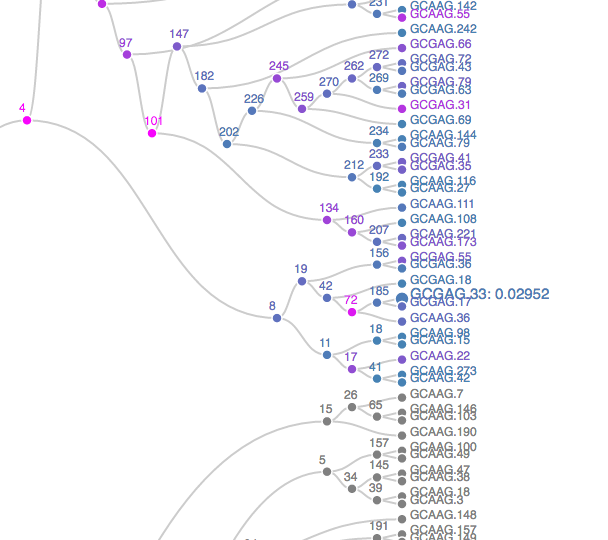
\includegraphics[scale=0.4]{figure/structssi-screenshot.png}
  \caption{A screenshot of a subtree with many differentially abundant
    bacteria, as determined by the hierarchical testing
    procedure. Currently the user is hovering over the node associated
    with bacteria GCGAG.33; this causes the adjusted $p$-value (0.0295)
    to appear.}
  \label{fig:structssi-hfdr}
\end{figure}

The plot opens in a new browser -- a static screenshot of a subtree is
displayed in Figure \ref{fig:structssi-hfdr}. Nodes are shaded
according to $p$-values, from blue to orange, representing the
strongest to weakest associations. Grey nodes were never
tested, to focus power on more promising subtrees. Scanning the full
tree, it becomes clear that the association between age group and
bacterial abundance is present in only a few isolated taxonomic
groups, but that it is quite strong in those groups. To give context
to these results, we can retrieve the taxonomic identity of the
rejected hypotheses.

\begin{knitrout}
\definecolor{shadecolor}{rgb}{0.969, 0.969, 0.969}\color{fgcolor}\begin{kframe}
\begin{alltt}
\hlkwd{options}\hlstd{(}\hlkwc{width}\hlstd{=}\hlnum{100}\hlstd{)}
\hlstd{tax} \hlkwb{<-} \hlkwd{tax_table}\hlstd{(pslog)[,} \hlkwd{c}\hlstd{(}\hlstr{"Family"}\hlstd{,} \hlstr{"Genus"}\hlstd{)]} \hlopt
  \hlkwd{data.frame}\hlstd{()}
\hlstd{tax}\hlopt{$}\hlstd{seq} \hlkwb{<-} \hlstd{short_names}

\hlstd{hfdr_res}\hlopt{@}\hlkwc{p.vals}\hlopt{$}\hlstd{seq} \hlkwb{<-} \hlkwd{rownames}\hlstd{(hfdr_res}\hlopt{@}\hlkwc{p.vals}\hlstd{)}
\hlstd{tax} \hlopt
  \hlkwd{left_join}\hlstd{(hfdr_res}\hlopt{@}\hlkwc{p.vals}\hlstd{)} \hlopt
  \hlkwd{arrange}\hlstd{(adjp)} \hlopt \hlkwd{head}\hlstd{(}\hlnum{10}\hlstd{)}
\end{alltt}
\begin{verbatim}
##                Family            Genus       seq   unadjp     adjp adj.significance
## 1     Lachnospiraceae        Roseburia  GCAAG.71 1.01e-67 2.02e-67              ***
## 2     Lachnospiraceae             <NA>  GCAAG.96 1.33e-67 2.65e-67              ***
## 3     Lachnospiraceae Clostridium_XlVa GCAAG.190 1.10e-58 2.21e-58              ***
## 4     Lachnospiraceae             <NA> GCAAG.254 2.01e-48 4.03e-48              ***
## 5     Lachnospiraceae Clostridium_XlVa GCAAG.150 4.90e-46 9.80e-46              ***
## 6  Porphyromonadaceae             <NA>   GCGAG.2 5.28e-38 1.06e-37              ***
## 7     Lachnospiraceae Clostridium_XlVa GCAAG.170 6.54e-38 1.31e-37              ***
## 8                <NA>             <NA>   GCAAG.1 1.16e-35 2.32e-35              ***
## 9     Lachnospiraceae             <NA> GCAAG.146 4.83e-33 9.66e-33              ***
## 10 Porphyromonadaceae             <NA>  GCGAG.21 1.40e-28 2.79e-28              ***
\end{verbatim}
\end{kframe}
\end{knitrout}

It seems that the most strongly associated bacteria all belong to
family \emph{Lachnospiraceae}, which is consistent with the random forest
results in Section \ref{sec:supervised-learning}.

\subsection*{Multitable techniques}

Many microbiome studies attempt to quantify variation in the
microbial, genomic, and metabolic measurements across different
experimental conditions. As a result, it is common to perform multiple
assays on the same biological samples and ask what features -- bacteria,
genes, or metabolites, for example -- are associated with different sample
conditions. There are many ways to approach these questions, which to
apply depends on the study's focus.

Here, we will focus on one specific workflow that uses sparse
Canonical Correlation Analysis (sparse CCA), a method well-suited to
both exploratory comparisons between samples and the identification of
features with interesting variation. We will use an implementation
from the  \CRANpkg{PMA} \cite{witten2009pma}.

Since the mouse data used above included only a single table, we use a
new data set, collected by the study
\cite{kashyap2013genetically}. There are two tables here, one for
bacteria and another with metabolites. 12 samples were obtained, each
with measurements at 637 m/z values and 20,609 OTUs; however, about
96\% of the entries of the microbial abundance table are exactly
zero. The code below retrieves this data.

\begin{knitrout}
\definecolor{shadecolor}{rgb}{0.969, 0.969, 0.969}\color{fgcolor}\begin{kframe}
\begin{alltt}
\hlkwd{setup_example}\hlstd{(}\hlkwd{c}\hlstd{(}\hlstr{"phyloseq"}\hlstd{,} \hlstr{"ggplot2"}\hlstd{,} \hlstr{"reshape2"}\hlstd{,} \hlstr{"ade4"}\hlstd{,} \hlstr{"PMA"}\hlstd{,}
                \hlstr{"genefilter"}\hlstd{,} \hlstr{"ggrepel"}\hlstd{))}

\hlstd{metab_path} \hlkwb{<-} \hlstr{"data/metabolites.csv"}
\hlstd{microbe_path} \hlkwb{<-} \hlstr{"data/microbe.rda"}
\hlstd{metab} \hlkwb{<-} \hlkwd{read.csv}\hlstd{(metab_path,} \hlkwc{row.names} \hlstd{=} \hlnum{1}\hlstd{)}
\hlstd{metab} \hlkwb{<-} \hlkwd{as.matrix}\hlstd{(metab)}
\hlstd{microbe} \hlkwb{<-} \hlkwd{get}\hlstd{(}\hlkwd{load}\hlstd{(microbe_path))}
\end{alltt}
\end{kframe}
\end{knitrout}

Our preprocessing mirrors that done for the mouse data. We first
filter down to microbes and metabolites of interest, removing those that
are zero across many samples. Then, we transform them to weaken the
heavy tails.

\begin{knitrout}
\definecolor{shadecolor}{rgb}{0.969, 0.969, 0.969}\color{fgcolor}\begin{kframe}
\begin{alltt}
\hlstd{keep_ix} \hlkwb{<-} \hlkwd{rowSums}\hlstd{(metab} \hlopt{==} \hlnum{0}\hlstd{)} \hlopt{<=} \hlnum{3}
\hlstd{metab} \hlkwb{<-} \hlstd{metab[keep_ix, ]}
\hlstd{microbe} \hlkwb{<-} \hlkwd{prune_taxa}\hlstd{(}\hlkwd{taxa_sums}\hlstd{(microbe)} \hlopt{>} \hlnum{4}\hlstd{, microbe)}
\hlstd{microbe} \hlkwb{<-} \hlkwd{filter_taxa}\hlstd{(microbe,} \hlkwd{filterfun}\hlstd{(}\hlkwd{kOverA}\hlstd{(}\hlnum{3}\hlstd{,} \hlnum{2}\hlstd{)),} \hlnum{TRUE}\hlstd{)}

\hlstd{metab} \hlkwb{<-} \hlkwd{log}\hlstd{(}\hlnum{1} \hlopt{+} \hlstd{metab,} \hlkwc{base} \hlstd{=} \hlnum{10}\hlstd{)}
\hlstd{X} \hlkwb{<-} \hlkwd{otu_table}\hlstd{(microbe)}\hlopt{@}\hlkwc{.Data}
\hlstd{X[X} \hlopt{>} \hlnum{50}\hlstd{]} \hlkwb{<-} \hlnum{50}
\end{alltt}
\end{kframe}
\end{knitrout}

We can now apply sparse CCA. This method compares sets of
features across high-dimensional data tables, where there may be
more measured features than samples. In the process, it chooses a
subset of available features that capture the most covariance -- these
are the features that reflect signals present across multiple
tables. We then apply PCA to this selected subset of features. In this
sense, we use sparse CCA as a screening procedure, rather than as an
ordination method.

Our implementation is below. The parameters \Robject{penaltyx} and
\Robject{penaltyz} are sparsity penalties. Larger values of
\Robject{penaltyx} will result in fewer selected  microbes, similarly
\Robject{penaltyz} modulates the number of selected metabolites. We
tune them manually to facilitate subsequent interpretation -- we
generally prefer more sparsity than the default parameters would
provide.

\begin{knitrout}
\definecolor{shadecolor}{rgb}{0.969, 0.969, 0.969}\color{fgcolor}\begin{kframe}
\begin{alltt}
\hlstd{cca_res} \hlkwb{<-} \hlkwd{CCA}\hlstd{(}\hlkwd{t}\hlstd{(X),}  \hlkwd{t}\hlstd{(metab),} \hlkwc{penaltyx} \hlstd{=} \hlnum{.15}\hlstd{,} \hlkwc{penaltyz} \hlstd{=} \hlnum{.15}\hlstd{)}
\end{alltt}
\begin{verbatim}
## 123456789101112131415
\end{verbatim}
\begin{alltt}
\hlstd{cca_res}
\end{alltt}
\begin{verbatim}
## Call: CCA(x = t(X), z = t(metab), penaltyx = 0.15, penaltyz = 0.15)
## 
## 
## Num non-zeros u's:  5 
## Num non-zeros v's:  15 
## Type of x:  standard 
## Type of z:  standard 
## Penalty for x: L1 bound is  0.15 
## Penalty for z: L1 bound is  0.15 
## Cor(Xu,Zv):  0.974
\end{verbatim}
\end{kframe}
\end{knitrout}

With these parameters, 5 microbes and 15 metabolites have been
selected, based on their ability to explain covariation between
tables. Further, these 20 features result in a correlation of
0.974 between the two tables. We interpret this
to mean that the microbial and metabolomic data reflect similar
underlying signals, and that these signals can be approximated well by
the 20 selected features. Be wary of the correlation value, however,
since the scores are far from the usual bivariate normal cloud.
Further, note that it is possible that other subsets of features could
explain the data just as well -- sparse CCA has minimized redundancy
across features, but makes no guarantee that these are the ``true''
features in any sense.

Nonetheless, we can still use these 20 features to compress
information from the two tables without much loss. To relate the
recovered metabolites and OTUs to characteristics of the samples on
which they were measured, we use them as input to an ordinary PCA.

\begin{knitrout}
\definecolor{shadecolor}{rgb}{0.969, 0.969, 0.969}\color{fgcolor}\begin{kframe}
\begin{alltt}
\hlstd{combined} \hlkwb{<-} \hlkwd{cbind}\hlstd{(}\hlkwd{t}\hlstd{(X[cca_res}\hlopt{$}\hlstd{u} \hlopt{!=} \hlnum{0}\hlstd{, ]),}
                  \hlkwd{t}\hlstd{(metab[cca_res}\hlopt{$}\hlstd{v} \hlopt{!=} \hlnum{0}\hlstd{, ]))}
\hlstd{pca_res} \hlkwb{<-} \hlkwd{dudi.pca}\hlstd{(combined,} \hlkwc{scannf} \hlstd{= F,} \hlkwc{nf} \hlstd{=} \hlnum{3}\hlstd{)}

\hlcom{# annotation}
\hlstd{genotype} \hlkwb{<-} \hlkwd{substr}\hlstd{(}\hlkwd{rownames}\hlstd{(pca_res}\hlopt{$}\hlstd{li),} \hlnum{1}\hlstd{,} \hlnum{2}\hlstd{)}
\hlstd{sample_type} \hlkwb{<-} \hlkwd{substr}\hlstd{(}\hlkwd{rownames}\hlstd{(pca_res}\hlopt{$}\hlstd{l1),} \hlnum{3}\hlstd{,} \hlnum{4}\hlstd{)}
\hlstd{feature_type} \hlkwb{<-} \hlkwd{grepl}\hlstd{(}\hlstr{"\textbackslash{}\textbackslash{}."}\hlstd{,} \hlkwd{colnames}\hlstd{(combined))}
\hlstd{feature_type} \hlkwb{<-} \hlkwd{ifelse}\hlstd{(feature_type,} \hlstr{"Metabolite"}\hlstd{,} \hlstr{"OTU"}\hlstd{)}

\hlstd{sample_info} \hlkwb{<-} \hlkwd{data.frame}\hlstd{(pca_res}\hlopt{$}\hlstd{li, genotype, sample_type)}
\hlstd{feature_info} \hlkwb{<-} \hlkwd{data.frame}\hlstd{(pca_res}\hlopt{$}\hlstd{c1,}
                           \hlkwc{feature} \hlstd{=} \hlkwd{substr}\hlstd{(}\hlkwd{colnames}\hlstd{(combined),} \hlnum{1}\hlstd{,} \hlnum{6}\hlstd{))}
\end{alltt}
\end{kframe}
\end{knitrout}

Figure \ref{fig:multitable-interpret-pca} displays a PCA {\em triplot}, where we show
different types of samples and the multidomain features (Metabolites and OTUs).
This allows comparison across the measured samples -- triangles for
Knockout and circles for wild type --
and characterizes the influence the different features  -- diamonds with
text labels. For example, we see that the main variation in the data
is across PD and ST samples, which correspond to the different diets.
Further, large values of 15 of the features are associated with ST
status, while small values for 5 of them indicate PD status. The
advantage of the sparse CCA screening is now clear -- we  can display
most of the variation across samples using a relatively simple plot,
and can avoid plotting the hundreds of additional points that would be
needed to display all of the features.

\begin{figure}[H]
\begin{knitrout}
\definecolor{shadecolor}{rgb}{0.969, 0.969, 0.969}\color{fgcolor}\begin{kframe}
\begin{alltt}
\hlkwd{ggplot}\hlstd{()} \hlopt{+}  \hlkwd{geom_point}\hlstd{(}\hlkwc{data} \hlstd{= sample_info,}
            \hlkwd{aes}\hlstd{(}\hlkwc{x} \hlstd{= Axis1,} \hlkwc{y} \hlstd{= Axis2,} \hlkwc{col} \hlstd{= sample_type,} \hlkwc{shape} \hlstd{= genotype),} \hlkwc{size} \hlstd{=} \hlnum{3}\hlstd{)} \hlopt{+}
  \hlkwd{geom_label_repel}\hlstd{(}\hlkwc{data} \hlstd{= feature_info,}
                   \hlkwd{aes}\hlstd{(}\hlkwc{x} \hlstd{=} \hlnum{5.5} \hlopt{*} \hlstd{CS1,} \hlkwc{y} \hlstd{=} \hlnum{5.5} \hlopt{*} \hlstd{CS2,} \hlkwc{label} \hlstd{= feature,} \hlkwc{fill} \hlstd{= feature_type),}
                   \hlkwc{size} \hlstd{=} \hlnum{2}\hlstd{,} \hlkwc{segment.size} \hlstd{=} \hlnum{0.3}\hlstd{,}
                   \hlkwc{label.padding} \hlstd{=} \hlkwd{unit}\hlstd{(}\hlnum{0.1}\hlstd{,} \hlstr{"lines"}\hlstd{),} \hlkwc{label.size} \hlstd{=} \hlnum{0}\hlstd{)} \hlopt{+}
  \hlkwd{geom_point}\hlstd{(}\hlkwc{data} \hlstd{= feature_info,}
             \hlkwd{aes}\hlstd{(}\hlkwc{x} \hlstd{=} \hlnum{5.5} \hlopt{*} \hlstd{CS1,} \hlkwc{y} \hlstd{=} \hlnum{5.5} \hlopt{*} \hlstd{CS2,} \hlkwc{fill} \hlstd{= feature_type),}
             \hlkwc{size} \hlstd{=} \hlnum{1}\hlstd{,} \hlkwc{shape} \hlstd{=} \hlnum{23}\hlstd{,} \hlkwc{col} \hlstd{=} \hlstr{"#383838"}\hlstd{)} \hlopt{+}
  \hlkwd{scale_color_brewer}\hlstd{(}\hlkwc{palette} \hlstd{=} \hlstr{"Set2"}\hlstd{)} \hlopt{+}
  \hlkwd{scale_fill_manual}\hlstd{(}\hlkwc{values} \hlstd{=} \hlkwd{c}\hlstd{(}\hlstr{"#a6d854"}\hlstd{,} \hlstr{"#e78ac3"}\hlstd{))} \hlopt{+}
  \hlkwd{guides}\hlstd{(}\hlkwc{fill} \hlstd{=} \hlkwd{guide_legend}\hlstd{(}\hlkwc{override.aes} \hlstd{=} \hlkwd{list}\hlstd{(}\hlkwc{shape} \hlstd{=} \hlnum{32}\hlstd{,} \hlkwc{size} \hlstd{=} \hlnum{0}\hlstd{)))} \hlopt{+}
  \hlkwd{coord_fixed}\hlstd{(}\hlkwd{sqrt}\hlstd{(pca_res}\hlopt{$}\hlstd{eig[}\hlnum{2}\hlstd{]} \hlopt{/} \hlstd{pca_res}\hlopt{$}\hlstd{eig[}\hlnum{2}\hlstd{]))} \hlopt{+}
  \hlkwd{labs}\hlstd{(}\hlkwc{x} \hlstd{=} \hlkwd{sprintf}\hlstd{(}\hlstr{"Axis1 [%s%% Variance]"}\hlstd{,}
                   \hlnum{100} \hlopt{*} \hlkwd{round}\hlstd{(pca_res}\hlopt{$}\hlstd{eig[}\hlnum{1}\hlstd{]} \hlopt{/} \hlkwd{sum}\hlstd{(pca_res}\hlopt{$}\hlstd{eig),} \hlnum{2}\hlstd{)),}
       \hlkwc{y} \hlstd{=} \hlkwd{sprintf}\hlstd{(}\hlstr{"Axis2 [%s%% Variance]"}\hlstd{,}
                   \hlnum{100} \hlopt{*} \hlkwd{round}\hlstd{(pca_res}\hlopt{$}\hlstd{eig[}\hlnum{2}\hlstd{]} \hlopt{/} \hlkwd{sum}\hlstd{(pca_res}\hlopt{$}\hlstd{eig),} \hlnum{2}\hlstd{)),}
       \hlkwc{fill} \hlstd{=} \hlstr{"Feature Type"}\hlstd{,} \hlkwc{col} \hlstd{=} \hlstr{"Sample Type"}\hlstd{)}
\end{alltt}
\end{kframe}

{\centering \includegraphics[width=\maxwidth]{analysisfigure/multitable-interpret-pca-1} 

}



\end{knitrout}
\caption{A PCA triplot produced from the CCA selected features in from muliple data types (metabolites and OTUs).
Note that we have departed from our convention of fixing the aspect ratio here as the second axis
represents very little of the variability and the plot would actually become unreadble.}
\label{fig:multitable-interpret-pca}
\end{figure}
